\documentclass[10pt]{article}

\usepackage[margin=0.75in, letterpaper]{geometry}
\usepackage{parskip}

\usepackage{amsthm, amsmath, amssymb}
\usepackage[pdftex]{graphicx}
\usepackage{hyperref}

\usepackage{enumerate} % For use of (a), (b), et cetera
\usepackage{booktabs} % Tables
\usepackage[margin=20pt, labelfont=bf, labelsep=period,
justification=justified]{caption} % Captions in figure floats

% https://stackoverflow.com/questions/3175105/inserting-code-in-this-latex-document-with-indentation
\usepackage{listings}
\usepackage{color}

% ======================
% Document setup, layout
% ======================

% Code block formatting
% http://texdoc.net/texmf-dist/doc/latex/listings/listings.pdf
\definecolor{dkgreen}{rgb}{0,0.6,0}
\definecolor{gray}{rgb}{0.5,0.5,0.5}
\definecolor{mauve}{rgb}{0.58,0,0.82}
\definecolor{lightgray}{rgb}{0.9,0.9,0.9}
\lstset{
  backgroundcolor=\color{lightgray},
  frame=none,
%  language=python,
  aboveskip=3mm,
  belowskip=3mm,
  showstringspaces=false,
  columns=flexible,
  basicstyle={\small\ttfamily},
  keepspaces=true,
  numbers=none,
  numberstyle=\tiny\color{gray},
  keywordstyle=\color{blue},
  commentstyle=\color{dkgreen},
  stringstyle=\color{mauve},
  breaklines=true,
  breakatwhitespace=true,
  tabsize=4,
%  mathescape=false,
}

% The following metadata will show up in the PDF properties
\hypersetup{
    colorlinks = true,
    urlcolor = magenta,  % Links to URLs
    linkcolor = blue,  % Links within PDF
    pdfauthor = {},
    pdfkeywords = {Torch, FLASH, AMUSE},
    pdftitle = {Torch Quick Start - \today},
    pdfsubject = {},
    pdfpagemode = UseNone
}

% Don't indent paragraphs
\setlength\parindent{0em}

% Slightly more compact lines
\linespread{0.95}

% ===============
% Useful commands
% ===============
\newcommand*{\mt}{\mathrm}
\newcommand*{\unit}[1]{\;\mt{#1}}  % vemod.net/typesetting-units-in-latex
\newcommand*{\abt}{\mathord{\sim}} % tex.stackexchange.com/q/55701
\newcommand*\mean[1]{\bar{#1}}
\renewcommand{\vec}[1]{\boldsymbol{#1}}  % Bold vectors
\newcommand*{\tsup}{\textsuperscript}
\newcommand*{\tab}{\hspace*{10mm}}

% Sets, operators
\newcommand*{\ints}{\mathbb{Z}}
\newcommand*{\ptl}{\partial}
\newcommand*{\dl}{\nabla}
\newcommand*{\dtl}{\mathrm{d}}

\newcommand*{\Msun}{M_\odot}
\newcommand*{\sun}{\odot}
\newcommand*{\kB}{k_\mathrm{B}}

\begin{document}

% =======
% Titling
% =======
\begin{center}
Torch Quick Start Guide \\
Last updated: \today \\
\end{center}

\tableofcontents
\newpage

% ==================================
% Introduction
% ==================================
\section{Introduction}

\textbf{Torch} is a star formation simulation code with magnetohydrodynamics
(FLASH), radiative transfer (Fervent), self-gravity \& sinks, star particles,
feedback (stellar winds, SNe), stellar evolution tracks (SeBa), and N-body
dynamics (AMUSE/PeTar).
Torch features and add-ons are listed in Figure~\ref{fig:features},
and references for the major components are in Appendix~\ref{sec:components}.

You can find a high-level overview of the code in:
\begin{itemize}
    \item Wall+ 2019, \href{https://arxiv.org/abs/1901.01132}{arXiv:1901.01132}
    \item Wall 2019, \href{https://www.dropbox.com/s/c0qh1no85y1jnxf/J_Wall-Thesis_final.pdf?dl=0}{Ph.D thesis}
\end{itemize}

Torch comprises (1) interface code that connects FLASH to AMUSE,
(2) a good number of add-on code units for FLASH, and (3) a set of Python scripts
that connect the codes and drive thes imulation.

To use Torch, you install additional code into FLASH, and then compile FLASH into an
AMUSE ``worker'' binary that enables FLASH to be called from AMUSE python scripts. You
then run a Python script to run the simulation.

\begin{figure}[!h]
    \center
    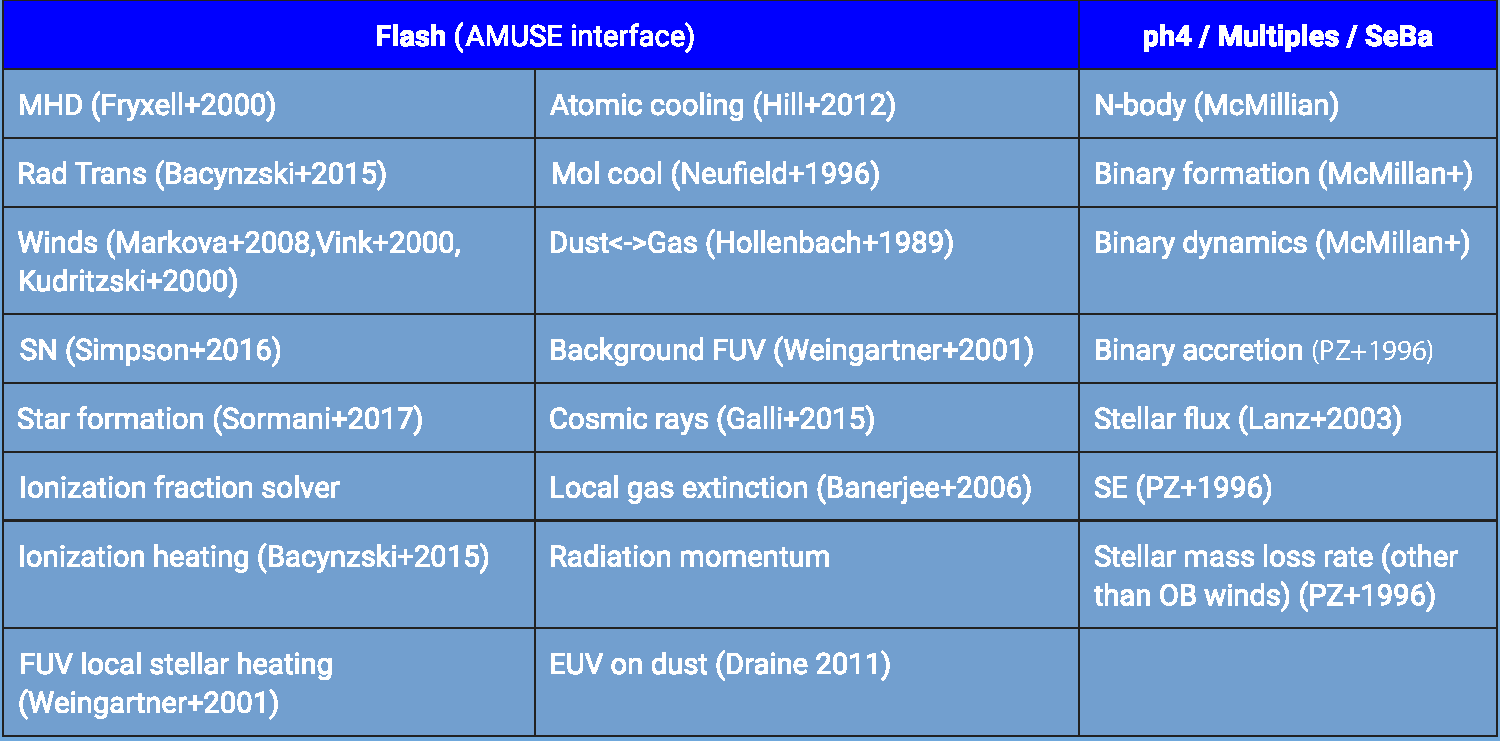
\includegraphics[width=0.9\textwidth]{fig/torch-features.pdf}
    \caption{
        Adapted from Wall+ 2018,
\href{https://cpb-us-e1.wpmucdn.com/sites.northwestern.edu/dist/d/1838/files/2018/07/Wall_MODEST18_Santorini-10rxnkm.pdf}{MODEST conference proceedings}
    }
    \label{fig:features}
\end{figure}

% ===========
% Quick Start
% ===========
\section{Quick Start}

Torch has many moving parts.  You'll likely have to adjust the procedure below
for your personal setup.  In any case, don't despair!  Torch has been
successfully built and run on a variety of systems.

We assume that you're using (1) the bash shell, and (2) conda or a virtualenv for Python
package management.  But, the setup procedure should work for any shell and
Python package manager with some adjustments.

% --------
% Overview
% --------

\subsection{Overview}

Torch consists of a collection of Fortran files that extend the FLASH MHD code, bindings
for AMUSE for that extended FLASH, and a set of Python scripts that use AMUSE to run a
simulation combining the extended FLASH with the other codes.

Installing Torch therefore entails 1) creating an environment and installing the
dependencies, including AMUSE, 2) installing Torch, with its extended FLASH and Python
parts, and 3) installing the FLASH AMUSE bindings to tie it all together.

% -----------
% Environment
% -----------

\subsection{Environment}

First, start a new shell session. You may want to check your \texttt{.bashrc} for any
old MPI or HDF5 configuration that could conflict with Torch setup -- module
load commands, environment variable exports, et cetera -- and comment them out.

Next, it is probably a good idea to make a project directory in which you can
download and install all the pieces:

\begin{lstlisting}[language=bash]
mkdir torch_project
\end{lstlisting}

You can call it something different or arrange the files differently if you want. In
particular if you're on an HPC cluster with a limited amount of space available in your
home directory, then you'll want to use another location instead, for example a scratch
directory. The documentation for the machine should tell you what is available. You'll
need about 2GB for the base installation, plus space for model output which can also
easily grow to multiple gigabytes.

Next, we'll need an environment to install the Python bits into, and possibly the native
tools and dependencies as well. There are two options here. If you're on an HPC machine,
then you'll probably want to use native tools and dependencies, and a Python virtual
environment for the Python bits. On a local machine, you can do that as well, or use
conda instead to get everything contained in a single environment. Both options are
described here.

\subsubsection{Local, with conda}

We'll assume here that you already have conda installed and available. If not, we
recommend installing the miniforge distribution from
\url{https://github.com/conda-forge/miniforge}.

First, we'll create and activate a new conda environment, and set it to use conda-forge:

\begin{lstlisting}[language=bash]
conda create -n Torch
conda activate Torch
\end{lstlisting}

Note that AMUSE is designed to work with the conda-forge package channel. Conda-forge
contains a very large variety of scientific and other packages, so you'll find
everything you need for Torch as well as other tools you may want to use.

Mixing conda channels is not recommended, as it leads to package incompatibilities, long
waits for the solver to try to deal with incongruent sets of packages when installing,
and hard to diagnose issues. So we strongly recommend sticking with conda-forge only.
Miniforge will do that by default.

If you open a new shell, then the environment needs to be reactivated using the
\texttt{conda activate Torch} command before you do anything else.

Once we have a conda environment, we can install the prerequisites inside of it, once
again making sure our packages come from conda-forge (some versions of conda can be a
bit stubborn on this):

\begin{lstlisting}[language=bash]
conda install -c conda-forge --override-channels pip wheel c-compiler cxx-compiler
fortran-compiler \ 'gfortran<14' python coreutils patch curl make openmpi hdf5 zlib
'docutils>=0.6' 'mpi4py>=1.1.0' \ 'numpy>=1.2.2' 'h5py>=1.1.0' scipy astropy jupyter pandas seaborn matplotlib yt
\end{lstlisting}

AMUSE is not yet available directly from conda-forge, so we'll have to install it from
source. First, we need to download and unpack it (into our project directory):

\begin{lstlisting}[language=bash]
curl -L -O "https://github.com/amusecode/amuse/archive/refs/tags/v2025.9.0.tar.gz"
tar xzf v2025.9.0.tar.gz
\end{lstlisting}

AMUSE has had a major upgrade to its installer recently, so be sure to get v2025.9.0 or
a later version, older ones won't work.

Next, we can move into the newly created AMUSE source directory, and run the installer:

\begin{lstlisting}[language=bash]
cd amuse-2025.9.0
./setup
\end{lstlisting}

This will produce quite a bit of output, including an overview of installable codes,
disabled codes and the reasons why, and follow-up instructions. If all went well then
you should now be able to install the AMUSE packages you need into your conda environment
using

\begin{lstlisting}[language=bash]
./setup install framework kepler petar ph4 seba smalln
\end{lstlisting}

Note that Torch doesn't necessarily use all of these, so if you know which ones you
want, then you can install only those. At any rate you can return to the AMUSE directory
later and use \texttt{./setup} to install more codes.

That concludes setting up the environment and the dependencies, so you can scroll past
the next section (one environment is enough, really!) and continue with installing
Torch.


\subsubsection{HPC, with virtualenv and modules}

As an alternative to Conda, you can also use a Python virtual environment to install the
Python dependencies into. Dependencies for the Fortran and C code in Torch will then
have to be installed in some other way. Linux computers typically have a built-in
package manager like \texttt{apt} or \texttt{dnf}, while on a Mac Homebrew and MacPorts
are commonly used. On HPC machines, you typically load the necessary modules.

If you're on a local machine and have one of the above package managers available, then
you should continue with the instructions below, but skip the loading of modules and
just make the virtual environment and install the Python dependencies into it. If you
then continue with installing AMUSE, the AMUSE installer will guide you through
installing the dependencies using whichever package manager you have available. (Note
that you won't need everything it suggests, because Torch doesn't use all of AMUSE. You
can save some disk space by limiting your selection.)

On an HPC cluster or similar environment, the main tools and dependencies are likely
already installed and available as modules. To use them, we'll have to activate them
using the \texttt{module} command.

First, let's see what's installed:

\begin{lstlisting}[language=bash]
module avail
\end{lstlisting}

This will show a long (potentially very long) list of installed packages, or modules.

On some systems, this will only show a few years, e.g. \texttt{2023 2024 2025}. In that
case, use \texttt{module load 2025} (the latest is usually best) and then try
\texttt{module avail} again to get the list.

Have a look through the list and see if you can find modules named \texttt{GCC},
\texttt{HDF5}, \texttt{OpenMPI} (or some other MPI implementation, like \texttt{MPICH}),
\texttt{make}, and \texttt{Python}. The exact names will vary from
machine to machine. If the list is long, it's better to let the computer search for you
using e.g. \texttt{module keyword HDF5}.

Often, there are multiple versions of a package available. The codes in Torch (and
AMUSE) are fairly old, so probably any version will work. If you see different packages
with names like \texttt{gompi} or \texttt{iimpi}, use the \texttt{gompi} ones, as those
match GCC and OpenMPI.

You may not need \texttt{make} if it's already available. If the command

\begin{lstlisting}[language=bash]
make --version
\end{lstlisting}

prints some text starting with GNU Make, then you're good to go.

Once you have found the needed module names, you can load the modules, for example for
Snellius using the 2025 software stack
(you'll need to modify the exact module names to suit your machine):

\begin{lstlisting}[language=bash]
module load 2025
module load GCC/14.2.0
module load OpenMPI/5.0.7-GCC-14.2.0
module load HDF5/1.14.6-gompi-2025a
module load make/4.4.1-GCCcore-14.2.0
module load Python/3.13.1-GCCcore-14.2.0
\end{lstlisting}

Next, we can make a Python virtual environment. This is a directory, which can go into
your project directory or wherever you want it.

\begin{lstlisting}[language=bash]
python3 -m venv /path/to/torch_project/Torch-env
\end{lstlisting}

We can then activate the environment, and install the Python dependencies:

\begin{lstlisting}[language=bash]
. /path/to/torch_project/Torch-env/bin/activate
pip3 install -U pip wheel scipy astropy jupyter pandas seaborn matplotlib yt
\end{lstlisting}


At this point, it's probably convenient to create a file you can load that will activate
the modules and the virtual environment whenever you want to work with Torch. To do
that, create a file named \texttt{Torch.env} in your project directory containing the
module load commands and the activation of the environment, like so:

\begin{lstlisting}[language=bash]
module load 2025
module load GCC/14.2.0
module load OpenMPI/5.0.7-GCC-14.2.0
module load HDF5/1.14.6-gompi-2025a
module load make/4.4.1-GCCcore-14.2.0
module load Python/3.13.1-GCCcore-14.2.0

. /path/to/torch_project/Torch-env/bin/activate
\end{lstlisting}

with appropriate modifications for your site. Now you can activate everything in one
command using \texttt{. Torch.env} in your project directory (note the period and the
space at the beginning, they're required).


With the environment set up and activated, we can install AMUSE and most of the codes
that Torch uses into it. First, we need to download and unpack it (into our project
directory):

\begin{lstlisting}[language=bash]
curl -L -O "https://github.com/amusecode/amuse/archive/refs/tags/v2025.9.0.tar.gz"
tar xzf v2025.9.0.tar.gz
\end{lstlisting}

AMUSE has had a major upgrade to its installer recently, so be sure to get v2025.9.0 or
a later version, older ones won't work.

Next, we can move into the newly created AMUSE source directory, and run the installer:

\begin{lstlisting}[language=bash]
cd amuse-2025.9.0
./setup
\end{lstlisting}

This will produce quite a bit of output, including an overview of installable codes,
disabled codes and the reasons why, and follow-up instructions.

If you're on a local machine and don't already have the dependencies installed, then
\texttt{./setup} will give you the required command to install them using your local
package manager. Note that you probably don't need all the dependencies it suggests
installing, as that is the complete set and Torch only uses a few of AMUSE's many codes.
Compilers for C, C++ and Fortran, MPI, HDF5, make and Python should go a long way.

If all went well then you should now be able to install the AMUSE packages you need into
your virtual environment using

\begin{lstlisting}[language=bash]
./setup install framework kepler petar ph4 seba smalln
\end{lstlisting}

Note that Torch doesn't necessarily use all of these, so if you know which ones you
want, then you can install only those. At any rate you can return to the AMUSE directory
later and use \texttt{./setup} to install more codes.

With that, we have a virtual environment that is ready to install Torch into.

% ----------------
% Installing Torch
% ----------------

\subsection{Installing Torch}

The first step to installing Torch is to get a copy of FLASH. To do that, you need to
register, which may take a few days, and then download FLASH 4.6.2. The FLASH homepage
(\url{http://flash.uchicago.edu/site/flashcode}) will show you how.

Once you have a \texttt{FLASH4.6.2.tar.gz} file in your project directory, you need to
unpack it, and then set the \texttt{FLASH\_DIR} environment variable so that the Torch
installer can find it:

\begin{lstlisting}[language=bash]
cd torch_project
tar xzf FLASH4.6.2.tar.gz
export FLASH_DIR=${PWD}/FLASH4.6.2
\end{lstlisting}

Running the most up-to-date version of Torch, with the VETTAM radiation solver, requires PETSc 3.19.x. 
Some HPC systems have the correct version of PETSc available as a module; if this is the case, load
PETSc and skip the step below. If the correct version of PETSc is not installed on your system,
you can download and compile it as follows:

\begin{lstlisting}[language=bash]
cd torch_project
wget https://ftp.mcs.anl.gov/pub/petsc/release-snapshots/petsc-3.19.6.tar.gz
tar -xvf petsc-3.19.6.tar.gz
cd petsc-3.19.6
./configure --with-cc=mpicc --with-cxx=mpic++ --with-fc=mpif90
\end{lstlisting}

You may need to specify the location of your HDF5 directory with the \texttt{--with-hdf5-dir} flag.
Once PETSc is compiled, the script will print instructions to make the code. Those will likely be
as follows:

\begin{lstlisting}[language=bash]
make PETSC_DIR=torch_project/petsc-3.19.6 PETSC_ARCH=arch-linux-c-debug all
make PETSC_DIR=torch_project/petsc-3.19.6 PETSC_ARCH=arch-linux-c-debug check
\end{lstlisting}

To ensure that Torch can find PETSc, add the following lines to your \texttt{Torch.env} file:

\begin{lstlisting}[language=bash]
export PETSC_DIR=torch_project/petsc-3.19.6 
export PETSC_ARCH=arch-linux-c-debug all
export LD_LIBRARY_PATH=${PETSC_DIR}/${PETSC_ARCH}/lib:$LD_LIBRARY_PATH
\end{lstlisting}

Next, we can download Torch, and set \texttt{TORCH\_DIR}:

\begin{lstlisting}[language=bash]
git clone https://bitbucket.org/torch-sf/torch.git
export TORCH_DIR=${PWD}/torch
\end{lstlisting}

Then we can move into the Torch directory, and run its installer:

\begin{lstlisting}[language=bash]
cd ${TORCH_DIR}
./install.sh
\end{lstlisting}

This will add the Fortran parts of Torch to FLASH. Next, we need to make the Python
parts of Torch available:

\begin{lstlisting}[language=bash]
export PYTHONPATH=$PYTHONPATH:$TORCH_DIR/src
\end{lstlisting}

You will want to add the exports of \texttt{TORCH\_DIR} and \texttt{FLASH\_DIR} to your
\texttt{Torch.env}, as well as the PYTHONPATH, like so:

\begin{lstlisting}[language=bash]
module load 2025
module load GCC/14.2.0
module load OpenMPI/5.0.7-GCC-14.2.0
module load HDF5/1.14.6-gompi-2025a
module load make/4.4.1-GCCcore-14.2.0
module load Python/3.13.1-GCCcore-14.2.0

. /path/to/torch_project/Torch-env/bin/activate

export PETSC_DIR=torch_project/petsc-3.19.6 
export PETSC_ARCH=arch-linux-c-debug all
export LD_LIBRARY_PATH=${PETSC_DIR}/${PETSC_ARCH}/lib:$LD_LIBRARY_PATH

FLASH_DIR=/path/to/FLASH4.6.2
TORCH_DIR=/path/to/torch

export PYTHONPATH=$PYTHONPATH:$TORCH_DIR/src
\end{lstlisting}

With Torch installed into FLASH, we can now go to the FLASH directory and configure it. We recommend
running with the VETTAM radiation solver:

\begin{lstlisting}[language=bash]
cd $FLASH_DIR
./setup Cube -auto -3d +amuseUSM +amuseMG +vettam +HandCnew +amuseSinksAndStars \
+amuseWind +enerinj +supportPPMupwind +pm4dev -maxblocks=100 +cube16 --site=torch_auto
\end{lstlisting}

You may also configure FLASH with the FERVENT radiation solver. It is significantly slower than VETTAM
for large numbers of sources, and we recommend that new users use VETTAM instead. If you want to use
FERVENT, for example to continue simulations run with a previous version of Torch, you can configure 
FLASH with:

\begin{lstlisting}[language=bash]
cd $FLASH_DIR
./setup Cube -auto -3d +amuseUSM +amuseMG +rayPE +HandCnew +amuseSinksAndStars \
+amuseWind +enerinj +supportPPMupwind +pm4dev -maxblocks=100 +cube16 --site=torch_auto
\end{lstlisting}

The final piece of the puzzle are Torch's AMUSE FLASH bindings. These make it possible
for the Python parts of Torch to talk to FLASH, including its Torch additions. Check
that you still have your virtual environment active, and then you can compile and
install FLASH and the bindings like this:

\begin{lstlisting}[language=bash]
cd $TORCH_DIR
make -C src/amuse/torch_amuse_flash develop-torch-amuse-flash
\end{lstlisting}

If you are recompiling after a failed attempt, make sure to clean the directory first:

\begin{lstlisting}[language=bash]
cd $TORCH_DIR
make -C src/amuse/torch_amuse_flash distclean
\end{lstlisting}

With that, your environment should contain a working Torch installation. Time to give
it a try!


%%%%%%%%%%%%%%%%%%%%%%%%%%%%%%%%%%%%%%%%%%%%%%

%
% \begin{lstlisting}[language=bash]
% export MPI_HOME=/path/to/openmpi-x.y.z
% export MPI_RUN=/path/to/openmpi-x.y.z/bin/mpirun
% export PATH=$MPI_HOME/bin:$PATH
% export MANPATH=$MPI_HOME/share/man:$MANPATH
% export LD_RUN_PATH=$MPI_HOME/lib:$LD_RUN_PATH
% export LD_LIBRARY_PATH=$MPI_HOME/lib:$LD_LIBRARY_PATH
% export CPATH=$MPI_HOME/include:$CPATH
%
% export HDF5_HOME=/path/to/hdf5-x.y.z
% export HDF5DIR=/path/to/hdf5-x.y.z/lib
% export HDF5INCLUDE=/path/to/hdf5-x.y.z/include
% export HDF5LIB="hdf5_fortran -lhdf5"
% export PATH=${HDF5_HOME}/bin:$PATH
% export LD_LIBRARY_PATH=${HDF5_HOME}/lib:$LD_LIBRARY_PATH
% export LD_RUN_PATH=${HDF5_HOME}/lib:$LD_RUN_PATH
% export LIBRARY_PATH=${HDF5_HOME}/lib:$LIBRARY_PATH
% export C_INCLUDE_PATH=${HDF5_HOME}/include:$C_INCLUDE_PATH
% export CPLUS_INCLUDE_PATH=${HDF5_HOME}/include:$CPLUS_INCLUDE_PATH
% \end{lstlisting}
%

%%%%%%%%%%%%%%%%%%%%%%%%%%%%%%%%%%%%%%%%%%%%%%

% --------------------
% Run Torch simulation
% --------------------
\subsection{Run a Torch simulation (Josh thesis Appendix B)}

You are now ready to run a Torch simulation!  We will simulate a
$3 \times 10^3 \Msun$, $5 \unit{pc}$ radius gas sphere in $\pm 7 \unit{pc}$
cubic domain with outflow boundary conditions.
In about a free-fall time ($\approx 2 \unit{Myr}$), the cloud will collapse
under its own gravity, create a sink particle, and begin forming stars.

Choose a directory for your simulation and \texttt{cd} there.  Then do:
\begin{lstlisting}[language=bash]
ln -s $TORCH_DIR/cool.dat
ln -s $TORCH_DIR/cube128
cp $TORCH_DIR/torch_user.py                torch_user.py
cp $TORCH_DIR/flash.par.turbsph_standard   flash.par
mkdir data
\end{lstlisting}

If you are running with VETTAM, make sure to also link the following files:
\begin{lstlisting}[language=bash]
ln -s $TORCH_DIR/src/flash/source/physics/materialProperties/Opacity/RadTrans/Semenov/*.dat ./
ln -s $TORCH_DIR/src/flash/source/physics/materialProperties/Opacity/RadTrans/Semenov/opacity.inp ./
\end{lstlisting}

The file \texttt{torch\_mainloop.py} is the heart of the simulation.  It
performs the split time-evolution with both FLASH and the n-body integrator
ph4 or PeTar, handles stellar evolution, and lots more. \texttt{torch\_user.py} is the main
source of control for users of Torch, where parameters can be set and initial stellar
conditions defined. 

The simulation should take 1--10 minutes to reach
$t_\mt{max} = 2 \unit{Myr} = 6.31 \times 10^{13} \unit{s}$.
It will use 7 threads: 2 for FLASH, 1+2 for n-body integration (ph4) and 
n-body binary interactions (multiples) or 1 for stellar dynamics (PeTar), 
1 for stellar evolution, and 1 for AMUSE itself.  At around $1 \unit{Myr}$, 
a sink particle will form and begin creating stars.  One or a few $\ge 7 \Msun$ 
stars may begin blowing a wind, so the time step may drop; you may wish 
to end the simulation early.

To run the simulation interactively, execute the command:
\begin{lstlisting}[language=bash]
mpiexec -n 1 python torch_user.py
\end{lstlisting}

On a compute cluster with Slurm, copy \texttt{run.sh} from the
\texttt{torch} repository to your simulation directory.
Edit the \texttt{SBATCH} options as needed.  Then do:
\begin{lstlisting}[language=bash]
sbatch run.sh
\end{lstlisting}
If you increase the number of tasks requested, \texttt{torch\_user.py}
will automatically assign more threads (workers) to FLASH.

Log files will be dumped in your current working directory, and simulation
outputs will be written to the \texttt{data/} directory.  If you re-start a
simulation, Torch (FLASH) will overwrite existing data, but append to (some)
existing logs.  You may want to rename or delete your old logs to help keep
track of your runs.

\begin{figure}
    \center
    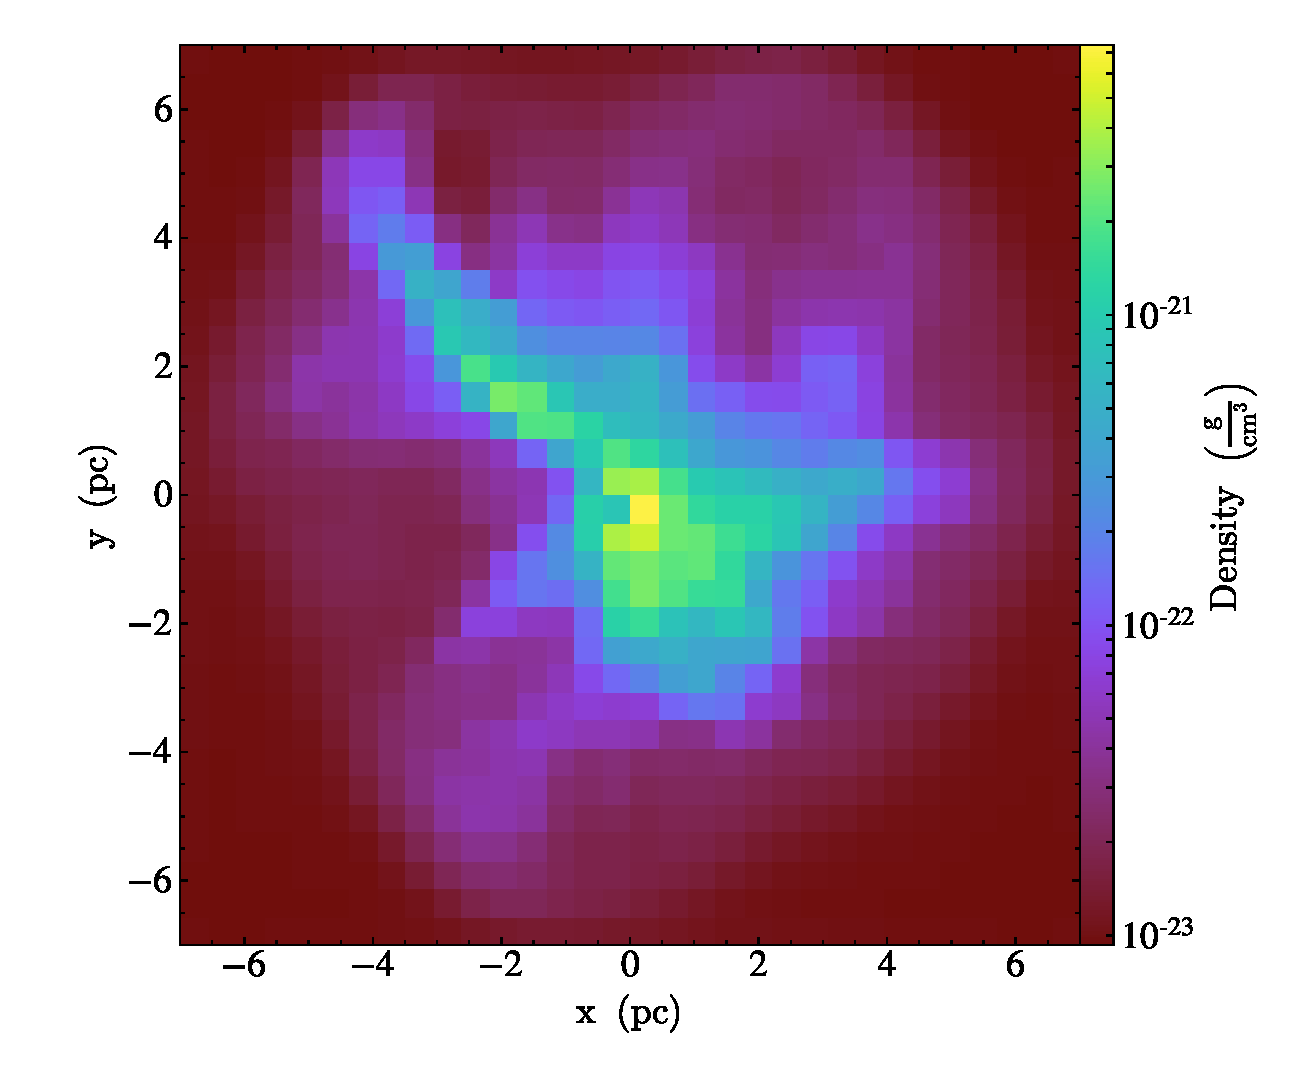
\includegraphics[width=0.5\textwidth]{fig/quickstart-dens-slice.pdf}
    \caption{
        Density in x-y plane.
    }
    \label{fig:dens}
\end{figure}

% ------------------
% Look at the output
% ------------------
\subsection{Look at the output}

Let's have a quick look at this gestating star cluster.  The example plots here
were created with the \texttt{yt} package, version 3.4.1.  To learn more about
\texttt{yt}, visit \url{http://yt-project.org/}.  To install \texttt{yt}:
\begin{lstlisting}[language=bash]
conda install yt
conda clean --all
\end{lstlisting}

We can first look at density-slice plots in the three coordinate planes (x-y,
x-z, y-z).  At the command line, call:
\begin{lstlisting}[language=bash]
yt plot data/turbsph_forced_hdf5_plt_cnt_0000
\end{lstlisting}
or, if you don't have a ``forced'' plot output, use the last ``plt\_cnt'' file
dumped by the simulation.
This will create a new directory \texttt{frames/} with three plots similar to
Figure~\ref{fig:dens}.

How about the particles?  Let's see how they're distributed, and inspect some
of their other properties.  In a Python session:
\begin{lstlisting}[language=python]
import numpy as np
import matplotlib.pyplot as plt
import yt

ds = yt.load('data/turbsph_hdf5_plt_cnt_0018')

ad = ds.all_data()
ppx = ad['all', 'particle_posx'].to('pc').value
ppy = ad['all', 'particle_posy'].to('pc').value
ppm = ad['all', 'particle_mass'].to('Msun').value
windy = ad['all', 'particle_dmdt'].value
windy[windy > 0] = 1

plt.scatter(ppx, ppy, s=ppm*6, c=windy, cmap='bwr', alpha=0.5)
plt.gca().set_aspect('equal')
plt.xlim(-2.5, +2.5)
plt.ylim(-2.5, +2.5)
plt.xlabel('x (pc)')
plt.ylabel('y (pc)')
plt.show()
\end{lstlisting}
In this particular simulation, three stars are massive enough to blow a wind
(Figure~\ref{fig:particles}).

\begin{figure}
    \center
    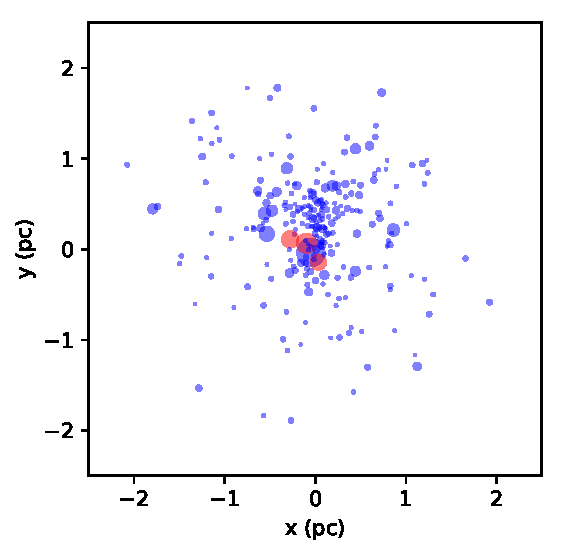
\includegraphics[width=0.4\textwidth]{fig/quickstart-particles.pdf}
    \caption{
        Star particles.  Size is proportional to mass; red particles have
        $\dtl m/\dtl t > 0$ (wind-blowing stars), blue particles have
        $\dtl m/\dtl t = 0$ (quiescent).
    }
    \label{fig:particles}
\end{figure}


% ----------
% Next steps
% ----------
\subsection{Next steps}

To tweak the simulation parameters, you will need to edit \texttt{flash.par}
and \texttt{torch\_user.py}.  These two files specify most of the
configuration options for the simulation.

%To understand how the initial gas-cloud conditions are set up, look at:
%\texttt{FLASH4.6.2/source/Simulation/SimulationMain/Cube/Simulation\_initBlock.F90}.

Torch comes packaged with a few simulations in
\texttt{FLASH4.6.2/source/Simulation/SimulationMain/}
\begin{verbatim}
    Cube
    EnergyInjection
    StratBox
\end{verbatim}
which provide initial conditions for (1) a turbulent gas sphere initialized
from a $128^3$ array, (2) a uniform medium for testing a stellar wind or
supernova, and (3) a planar gas layer in a periodic domain, driven by random
thermal supernova explosions.

It's often useful to reduce the number of Torch features for study or
debugging.  Below are setup calls showing some reduced feature sets:

Full Torch code with AMUSE/FLASH coupling.
\begin{lstlisting}[language=bash]
./setup Cube -a -3d +amuseUSM +amuseMG +rayPE +HandCnew +amuseSinksAndStars \
	+amuseWind +enerinj +supportPPMupwind +pm4dev -maxblocks=100 +cube16
\end{lstlisting}

FLASH-only simulation, no AMUSE coupling. Sinks will work, but no stars will
form.
\begin{lstlisting}[language=bash]
./setup Cube -a -3d +usm +gravMgrid +rayPE +HandCnew  +amuseSinksAndStars \
    +amuseWind +enerinj +supportPPMupwind +pm4dev -maxblocks=100 +cube16
\end{lstlisting}

FLASH-only simulation, no ray-tracing or sinks/stars.  Only self-gravity and
heating/cooling.
\begin{lstlisting}[language=bash]
./setup Cube -a -3d +usm +gravMgrid +HandCnew \
	+supportPPMupwind +pm4dev -maxblocks=100 +cube16
\end{lstlisting}

FLASH-only simulation, only MHD.
\begin{lstlisting}[language=bash]
./setup Cube -a -3d +usm +supportPPMupwind +pm4dev -maxblocks=100 +cube16
\end{lstlisting}

Note that \texttt{+rayPE} generally requires \texttt{+amuseSinksAndStars}.
These setup flags are aliases for various FLASH units; the flags are defined in
\texttt{FLASH4.6.2/bin/setup\_shortcuts.txt}.

Don't forget that after a fresh setup + compile of FLASH, you will need to
recompile the AMUSE worker too.

% ==========================
% Additional physics modules
% ==========================
\section{Parameters Choices \& Default Values}

% ============
%     PeTar
% ============
\subsection{PeTar Stellar Dynamics}

Torch is now capable of using \texttt{PeTar} for stellar dynamics. This is recommended for all runs, but particularly for runs with $>5,000$ stars or runs containing many binaries such as those with primordial binaries. To use \texttt{PeTar}, set
\begin{lstlisting}[language=python]
p['with_petar'] = True
p['r_bin'] = 100 | units.au
p['r_out'] = 0.03 | units.pc # outer radius for tree 
p['dt_soft_max'] = 0.125 | units.kyr # maximum PeTar timestep
\end{lstlisting}
in \texttt{torch\_user.py}. \texttt{PeTar} accepts the user parameter \texttt{r\_out} which is a boundary radius between the tree gravity and direct N-body and SDAR. 
For a thorough understanding of the parameters used in \texttt{PeTar}, users should familiarize themselves with the \href{https://github.com/lwang-astro/PeTar}{README} of the \texttt{PeTar} github and the \texttt{PeTar} \href{https://ui.adsabs.harvard.edu/abs/2020MNRAS.497..536W/abstract}{methods paper}.
\texttt{r\_out} and \texttt{dt\_soft\_max} must be set together, to ensure that dynamics are properly resolved at all separations. In the plot below, the different combinations have been chosen for
binaries with masses 1 M$_{\odot}$ and 0.1 M$_{\odot}$, and correspond to the timestep and \texttt{r\_out} for which an orbit is resolved by 10 or 100 steps, at \texttt{r\_out} or \texttt{r\_in}.
The recommended usage is to pick a combination of timestep and \texttt{r\_out} along or below the red line, which ensures that orbits with separation \texttt{r\_in} are resolved by 100 steps. 
The default values (0.03 pc and 125 yr) are shown as the black star, and were chosen to match the upper limit of a FLASH timestep once feedback stars have formed, at a resolution around 0.1-0.2 pc.
\begin{figure}[!h]
    \center
    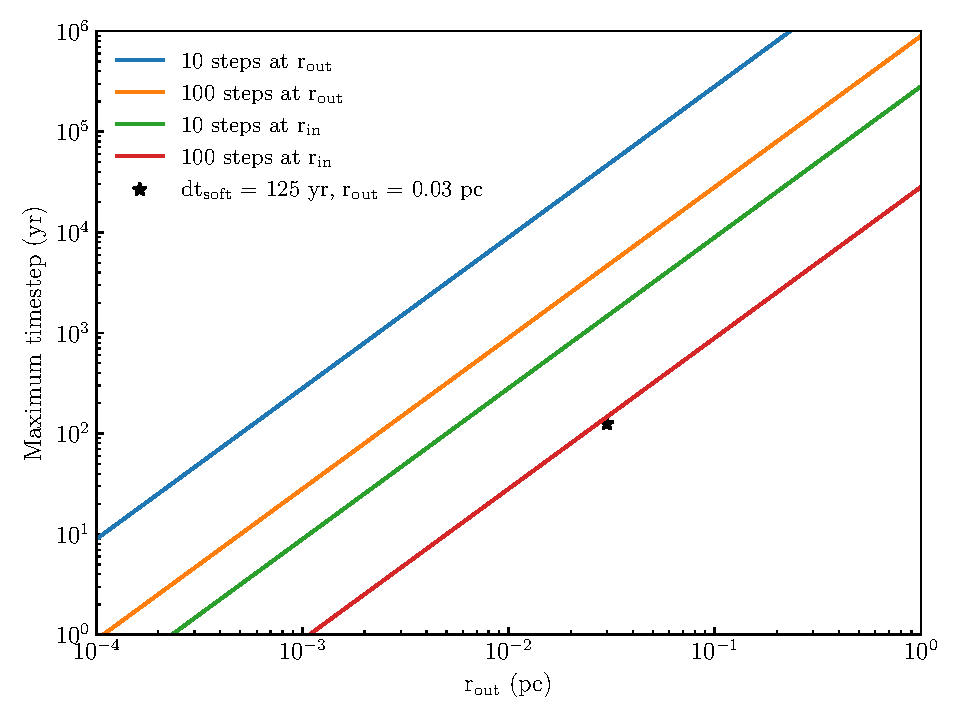
\includegraphics[width=0.7\textwidth]{fig/petar_dt.pdf}
    \label{fig:petar_dt}
\end{figure}

\subsection{VETTAM Radiation Solver}
\textbf{Additional documentation on the choice of VETTAM parameters to be added here before merging \texttt{develop} into \texttt{main}. If you are not familiar with VETTAM, use the defaults from \texttt{flash.par.turbsph\_standard}.}

\subsection{Primordial Binaries}

The primordial binaries implemented in this branch are based on observations compiled by Moe \& Di Stefano (2017) for solar-type and early-type stars, and on the observations by Winters et al. (2019, as corrected by Offner et al. 2023) 
for low-mass stars. The sampling routine for binaries is stored in \texttt{primordial\_binaries.py}, which can be readily modified to allow for other prescriptions. The values in the present version however reflect the mass-dependent binary 
fraction observed for main sequence stars, as well as the mass-dependent period distribution, and the mass- and period-dependent mass ratio and eccentricity distributions. Those distributions are shown in the plots below.

\begin{figure}[h!]
\centering
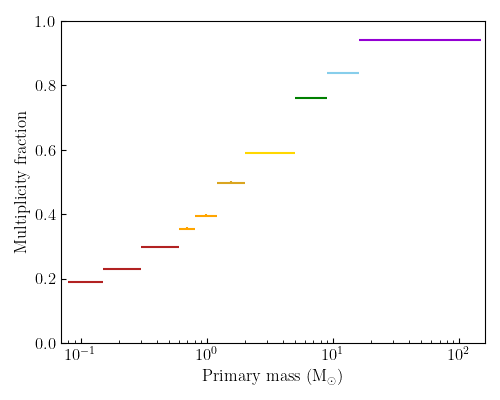
\includegraphics[width=0.5\linewidth]{fig/binary_frac.png}
\label{fig:binary_frac}
\caption{Binary fraction as a function of primary mass, based on the multiple star fractions reported in \href{https://ui.adsabs.harvard.edu/abs/2017ApJS..230...15M/abstract}{Moe \& Di Stefano (2017)} 
and \href{https://ui.adsabs.harvard.edu/abs/2023ASPC..534..275O/abstract}{Offner+ (2023)}.}
\end{figure}

\begin{figure}[h!]
\centering
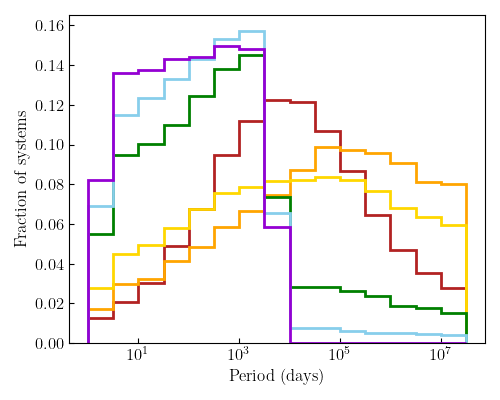
\includegraphics[width=0.5\linewidth]{fig/binary_period.png}
\label{fig:binary_period}
\caption{Binary period distribution for each mass range shown above. The distributions are from \href{https://ui.adsabs.harvard.edu/abs/2017ApJS..230...15M/abstract}{Moe \& Di Stefano (2017)} 
and \href{https://ui.adsabs.harvard.edu/abs/2023ASPC..534..275O/abstract}{Offner+ (2023)}.}
\end{figure}

\begin{figure}[h!]
\centering
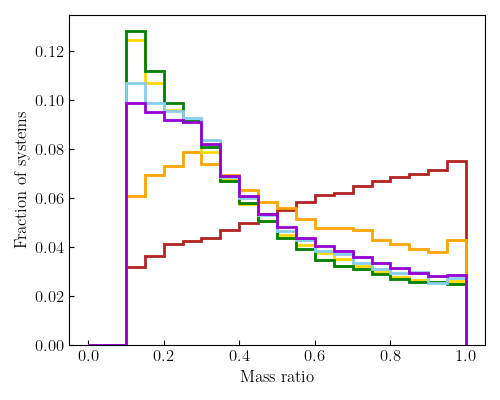
\includegraphics[width=0.5\linewidth]{fig/binary_mrat.png}
\label{fig:binary_mass_ratio}
\caption{Binary mass ratio distribution for each mass range shown above. The distributions are from \href{https://ui.adsabs.harvard.edu/abs/2017ApJS..230...15M/abstract}{Moe \& Di Stefano (2017)} and 
\href{https://ui.adsabs.harvard.edu/abs/2023ASPC..534..275O/abstract}{Offner+ (2023)}, and depend on both primary mass and orbital period.}
\end{figure}

\begin{figure}[h!]
\centering
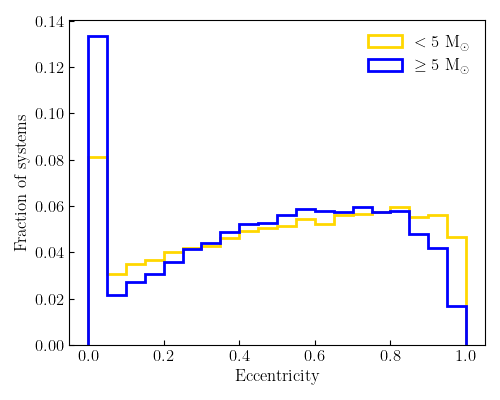
\includegraphics[width=0.5\linewidth]{fig/binary_ecc.png}
\label{fig:binary_eccentricity}
\caption{Binary eccentricity distribution as a function of primary mass, from \href{https://ui.adsabs.harvard.edu/abs/2017ApJS..230...15M/abstract}{Moe \& Di Stefano (2017)}.}
\end{figure}

To use primordial binaries in your simulations, the following parameters must be set in \texttt{torch\_user.py}:
\begin{lstlisting}[language=python]
p['binaries'] = True
# Not used if binaries is false, can leave to default values                                                                
p['mult_frac'] = 'field'  #Currently accepted method is 'field'.
p['pdist'] = 'inner' #Currently accepted methods are 'field' and 'inner'. 
p['qdist'] = 'field' #Currently accepted method is 'field'. 
p['edist'] = 'field' #Currently accepted method is 'field'. 
\end{lstlisting}
The recommended value for the period distribution is 'inner', which is designed to sample the inner companion in hierarchical triples while 'field' samples a random companion. The 'inner' distribution better reproduces the observed
close binary population. This choice is most important for massive stars, which have both a large triple fraction and a large fraction of systems with close companions. 

\subsection{Interacting Binaries}
To use interacting binaries in your simulations, the following parameters must be set in \texttt{torch\_user.py}:
\begin{lstlisting}[language=python]
p['with_be'] = True
p['massloss_method'] = 'seba-puls'
p['remove_merged'] = True
p['binaries'] = True # can be set to False, not recommended
# Feedback channels, interacting binaries have not been tested when those are turned off
p['with_lyc'] = True
p['with_pe_heat'] = True
p['with_sn'] = True
p['with_winds'] = True
\end{lstlisting}
Note that the \texttt{p['min\_feedback\_mass']} parameter now sets the minimum feedback for the primary in a binary system; if the companion is less massive than this mass, the system will still produce feedback.


% ============
% VorAMR Addon
% ============
\section{VorAMR: Expanded Options for Initial Conditions}
A normal Torch run initializes from a "cubefile" like \texttt{cube128} or one generated from \texttt{turb-sphere.py}. These initial conditions are currently restricted to spherical clouds with a turbulent velocity distribution and gaussian density profile or something similar. While such ICs make for easy first steps for users to setup a new Torch simulation, ideal ICs would come from systems that evolved self-consistently in galactic environments. 

\texttt{VorAMR} was created to allow for output data from other star formation software suites to be used as initial conditions in Torch. Currently, \texttt{VorAMR} has only been shown to be able to convert data from the star formation code \texttt{AREPO} into Torch ICs, but in theory can be easily adapted to convert ANY moving-mesh, AMR, or SPH code into Torch ICs.

\subsection{How VorAMR works}
\begin{figure}[!h]
    \center
    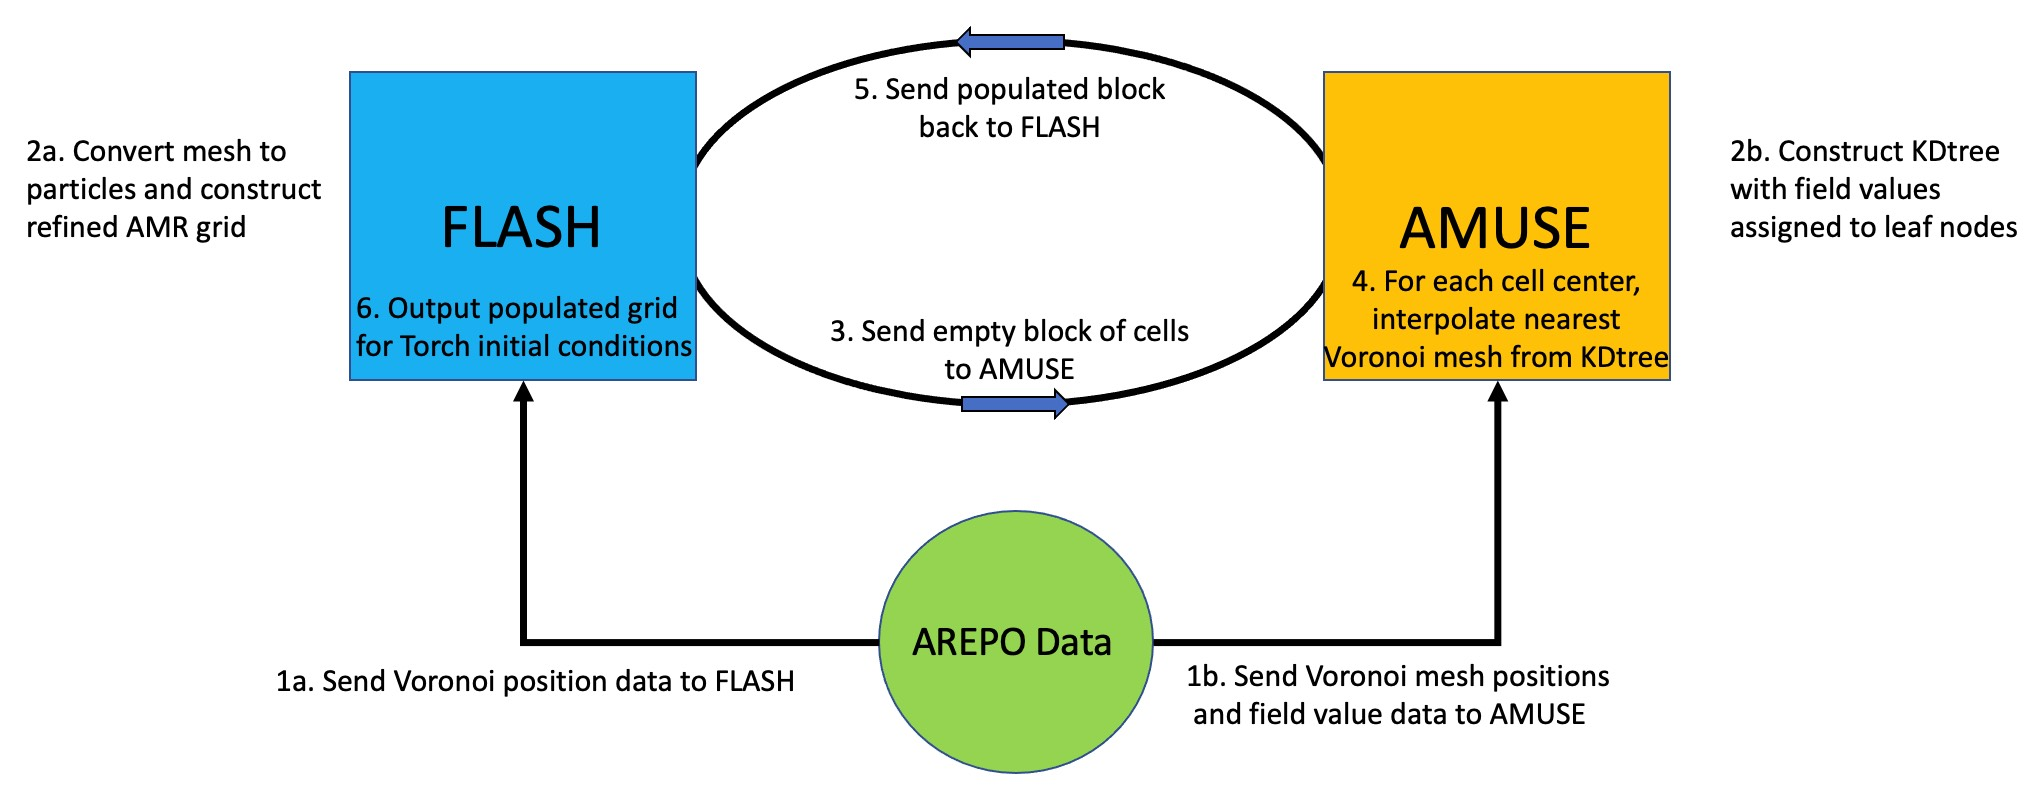
\includegraphics[width=0.9\textwidth]{fig/voramr_logic.jpeg}
    \caption{VorAMR logic flow.}
    \label{fig:voramr}
\end{figure}

\texttt{VorAMR} uses output data from other hydro-codes to build a refined grid in \texttt{FLASH} and then populate that grid with field values (density, internal energy, velocity, etc.) via the \texttt{AMUSE} interface. By doing this all within the Torch framework, the resulting grid and initial gas/particle properties allows Torch to immediately launch into a simulation but with external data as its initial conditions.

\texttt{VorAMR} takes advantage of the "refine\_on\_particle" routines within \texttt{FLASH} to construct a refined grid that as accurately as possible mirrors the local mesh scale of the \texttt{AREPO} data. \texttt{VorAMR} also uses a nearest-neighbor NDInterpolator to fill the \texttt{FLASH} grid cells with the field data of the nearest Voronoi mesh element (and therefore the element which encapsulates the cell center).

\subsection{How to use VorAMR}

\texttt{VorAMR} is installed alongside Torch but is turned off by default; Torch operates normally with \texttt{VorAMR} turned off. 
To turn \texttt{VorAMR} on, switches must be flipped in the flash.par file. Note, the file \texttt{flash.par.turbsph\_standard} does not have \texttt{VorAMR} switches, \texttt{flash.par.voramr} is meant to be identical but with the \texttt{VorAMR} switches included.

\begin{lstlisting}[language=bash]
# ================
# VorAMR extension
# ================
use_voramr = .true. # main control switch
voramr_source = "snapshot_518_9.hdf5" # source data to be converted
voramr_input = "voramr_input.hdf5" # name of file to be read-in by FLASH

refine_on_particle_count = .true. # builds grid based on source data - BE SURE TO TURN OFF FOR NORMAL TORCH
min_particles_per_blk    = 4096 # Assumes 16x16x16 blocks
max_particles_per_blk    = 4096 
pt_maxPerProc            = 10000000 # Enough to fit all particles on one proc - CAN BE REDUCED FOR NORMAL TORCH
refineonjeanslength = .true. 

# Restrict initial refinement by only placing particles within radius 
use_localRef = .false. 
center_localRef = .false. # Crops FLASH domain centered at localRef_{x,y,z} and centers new domain
# Local refinement center and radius
localRef_x = 3.20621187e+20 # cm
localRef_y = 6.24367575e+20
localRef_z = -1.51873194e+20
localRef_r = 1.543e+20

# Background Potential
sim_withStaticGrav = .true.
              # AREPO 518_9   # Hill et al 2012
sim_aParm1  = 1.31142525e-72  #4.39996789e-9  # [cm/s^2]     # 1.42E-3 [kpc/Myr^2]
sim_aParm2  = 1.35401904e-52  #5.51293615e-31 # [1/s^2]      # 5.49E-4 [1/Myr^2]
sim_aParm3  = -2.36078509e-30 #5.55421965e20  # [cm]         # 0.18E0  [kpc]
sim_aParm4  = 4.06112841e-11  #1.62715932e-53 # [1/(cm s^2)] #5 .0E-5  [1/kpc Myr^2]
\end{lstlisting}

Some of these switches are reflected in the \texttt{torch\_user.py} file, all \texttt{flashp[`..']} data is extracted directly from \texttt{flash.par}:

\begin{lstlisting}[language=python]
    p = {}
    flashp = FlashPar("flash.par")

    # <VorAMR>

    p['with_voramr'] = flashp['use_voramr']
    p['source_file'] = flashp['voramr_source']
    p['convert_file'] = True # Runs source_file through src/voramr/hdf5_convert.py 
    p['use_localRef'] = flashp['use_localRef']
    p['local_ref'] = [flashp['localRef_x'], flashp['localRef_y'], flashp['localRef_z'], flashp['localRef_r']]
    p['center_local_ref'] = flashp['center_localRef']
    p['input_file'] = flashp['voramr_input']
    p['pickle_kdtree'] = False # saves kdtree built from source_file used in interpolation. Useful if memory strained.
    p['pickle_file_name'] = "kdtree.pickle"
    p['numBlocks'] = 15000 # Quirky parameter, just set to any number larger than total num actual blocks and FLASH will figure it out.
    p['cellsPerBlock'] = 16
\end{lstlisting}

Once \texttt{VorAMR} is turned on, install torch as normal \texttt{. ./install.sh}.

Then, setup FLASH with enough MAXBLOCKS to allow for the expected refined grid to fit on a single processor. 

\begin{lstlisting}[language=bash]
./setup Cube -a -3d +amuseUSM +amuseMG +rayPE +HandCnew +amuseSinksAndStars \
	+amuseWind +enerinj +supportPPMupwind +pm4dev -maxblocks=10000 +cube16
\end{lstlisting}

Change the `lrefine\_max` value in flash.par to be whatever level you wish the grid to reach at its highest refinement regions. To acheive maximum consistency with the structure of the input data, `lrefine\_max` should be set such that the highest refinement FLASH blocks will contain as many input data points as cells (4096 for +cube16 blocks).

If your source data contains star particles that you would like to include in Torch, edit \texttt{user\_initial\_conditions()} in \texttt{torch\_user.py} to read in the particle data, incorporate them into an \texttt{AMUSE} particle set, and initialize them via the \texttt{hydro} class.

It is then recommended to change the following \texttt{flash.par} parameters to force \texttt{VorAMR} to output a checkpoint file as fast as possible. That resulting checkpoint can the be restarted from with \texttt{VorAMR} turned off.

\begin{lstlisting}[language=bash]
tmax            = 6.30e8 # two init timesteps 
dtinit          = 3.15e8
dtmin           = 3.15e7

checkpointFileIntervalTime  = 3.15e7 # dt_min
plotFileIntervalTime        = 3.15e8
particleFileIntervalTime    = 3.15e8 
\end{lstlisting}

Finally, run Torch with only 1 processor assigned to \texttt{flash\_worker} (if running default worker partitions, this would be 6 total processors: 1 driver, 2 \texttt{ph4}, 1 \texttt{SeBa}, 1 \texttt{multiples}, 1 \texttt{FLASH}). Note, when restarting from a \texttt{VorAMR} checkpoint, any number of processors can be used as long as \texttt{use\_voramr = .false.}

In addition to the usual Torch output, \texttt{VorAMR} produces two more files:
\begin{enumerate}
	\item \texttt{voramr\_input.hdf5} - the particle data extracted from the source data. This is what \texttt{FLASH} sees and will refine on.
	\item \texttt{interp-data.hdf5} - the file from which the interpolation kdtree is built. Only \texttt{AMUSE} sees this file, but then passes info from it to \texttt{FLASH}. This file will always contain all data from the source file.
\end{enumerate}
These files are both produced as sometimes we only want \texttt{FLASH} to refine on a portion of the source data, but we want \texttt{AMUSE} to have an accurate kdtree for all data to avoid domain edge effects during interpolation.

\subsection{Regional Refinement}

Torch is capable of de-refining the grid to a user defined level outside of a user defined rectangular region of interest. This is most useful in large-scale runs such as those initialized with \texttt{VorAMR}. To use this capability, the user must set the parameters listed below in the \texttt{flash.par} file. 

\begin{lstlisting}[language=bash]
# ===================================================
# Derefinement outside rectangular region of interest
# ===================================================
use_deref         = .true.
deref_lref        = 2  # level to derefine to
# EXAMPLE: derefine to level deref_lref outside center 5pc square
deref_xl          = -1.543e+19  # 5pc
deref_xr          =  1.543e+19 
deref_yl          = -1.543e+19
deref_yr          =  1.543e+19
deref_zl          = -1.543e+19
deref_zr          =  1.543e+19
\end{lstlisting}


% ============
% Known Issues
% ============
\section{Caveats and Known Issues}
\label{sec:caveats}

\subsection{Torch Issues}
Unphysical hot/empty zones are a common problem in finite volume codes, and are
readily generated by under-resolved supernovae and stellar winds in Torch.  To
combat such zones, a few tactics include:
\begin{itemize}
    \item Lower CFL
    \item Restart with more diffusive hydro solver parameters, temporarily
    \item Manually smooth out extremely sharp gradients
    \item Enable or increase artificial shock viscosity.
    \item Use the time-step limiter for positive-definite cell values (already
        enabled in the example Torch flash.par files).  This is controlled by
        the FLASH runtime parameter \texttt{dr\_usePosdefComputeDt}, among
        others.
    \item \texttt{VorAMR} is currently hardcoded to extract data from and refine on data from AREPO file structures. To change to other file structures, edits will need to be made to at least \texttt{src/voramr/hdf5\_convert.py} and possibly \texttt{src/flash/source/Simulation/SimulationMain/Cube/pt\_initVoronoiPositions.F90}
\end{itemize}
See \url{http://flash.uchicago.edu/pipermail/flash-users/2019-May/002908.html}
for a nice explanation by Sasha Tchekhovskoy.

%If using old AMUSE commit (?) with OpenMPI-4.0.0, will get C++ bindings error.
%Needs Josh fix.  Non-issue if we can move forward with new AMUSE.

In the FLASH unsplit solver, the logic for the hybrid Riemann solver is
slightly altered; see the \texttt{torch} file: \\
\texttt{src/flash/source/physics/Hydro/HydroMain/unsplit/hy\_uhd\_dataReconstOneStep.F90}

Torch does not support the use of BHTree with AMUSE.  Code exists to hook
FLASH/BHTree and AMUSE together, but it needs a small update and some testing
to work.

Several add-on ParticleInitialization, ParticleMapping, etc. units are provided
with Torch.  These were created to trace supernova and superbubble ejecta in
stratified box simulations run by Ibanez-Mejia et al.
(\href{https://iopscience.iop.org/article/10.3847/1538-4357/aa93fe}{2017}).
However, these have not been tested with the Torch sink/star framework and
probably will not work correctly as is.

The module \texttt{source/physics/sourceTerms/GridInject} is in development and
not recommended for use yet.

\subsection{VorAMR Issues}
\texttt{VorAMR} is capable of building Torch-ready initial conditions from ANY hydrodynamical simulation output. But, \texttt{VorAMR} is limited in how quickly it can complete this process. Luckily, a user will only have to use VorAMR once for a major production run, so the initial cost of time is generally worthwhile.
\begin{itemize}
	\item \texttt{VorAMR} can only run with ONE oversubscribed processor for the \texttt{flash\_worker} due to the use of serial HDF5 open/read calls within \texttt{FLASH}. Data conversion and grid build times can be on the order of days.
	\item Users are recommended to augment a Torch+\texttt{VorAMR} run to output a checkpoint file after ONE timestep. Then, restart from the checkpoint in a clean Torch build without \texttt{VorAMR} turned on.
	\item Sometimes \texttt{VorAMR} will run fine, but the resulting grid does not appear to be refined. Check in \texttt{turbsph.log} and see if the number of particles reported matches the dimensions of the array sent so FLASH (reported in slurm file) and what FLASH actually reads (reported in flash\_worker.out). If there is a mismatch, then it's likely that some refinement particles are being placed outside of the computational domain. Make sure your domain dimensions correctly reflect the source data.
\end{itemize}

% ===========
% Help!
% ===========
\section{Help!}
%\label{sec:help}

% ---------------
% General remarks
% ---------------
\subsection{General checks}

\begin{itemize}

    \item Are all packages built using the same compiler set?

    \item Check your environment variables.  Is PATH pointing somewhere it
        shouldn't?  Are two different installs/versions of a module visible in
        PATH?

    \item Anaconda or Conda may provide its own HDF5.  If you are using this
        HDF5, great, but if you are using a system HDF5 install, not so great.
        Check your PATH and make sure that the desired system HDF5 comes before
        the Anaconda/Conda HDF5.

    \item Check that FLASH, AMUSE, and mpi4py are using the same HDF5 and MPI
        libraries.

    \item If you had to swap MPI modules and reinstall \texttt{mpi4py} at any
        point, \texttt{pip install} needs the \texttt{--no-cache-dir} flag or
        else \texttt{mpi4py}'s compiled object library will not be reinstalled.
        You can check that \texttt{mpi4py} is linked to the correct MPI library
        by doing:

\begin{lstlisting}[language=bash]
ldd {your/conda_env/directory}/{env_name}/lib/python2.7/site-packages/mpi4py/MPI.so
\end{lstlisting}

    \item Here are some commands that may help diagnose library and path problems:

\begin{lstlisting}[language=bash]
module list
module show some/module/name
which python
which mpiexec
python -c "from mpi4py import MPI; print MPI"
ldd flash4
ldd flash_worker
\end{lstlisting}

\end{itemize}

% --------------
% FLASH problems
% --------------
\subsection{FLASH setup/compile problems}
%\label{sec:help-flash}

\begin{itemize}

    \item \textbf{make fails immediately with something like
        \texttt{/usr/local/mpich2//bin/mpif90: Command not found}.}

        Check that you are using the correct \texttt{Makefile.h}, with
        \texttt{MPI\_PATH} and \texttt{HDF5\_PATH} appropriate for your system.

    \item \textbf{make is slow.}

        Try \texttt{make -j} to use multiple processes.

    \item \textbf{make succeeds, but flash4 or flash\_worker fails at runtime with
        error like \texttt{error while loading shared libraries: libhdf5.so.8:
        cannot open shared object file}.}

        Take a look at \url{http://flash.uchicago.edu/pipermail/flash-users/2013-July/001322.html}.

    \item \textbf{FLASH runs out of memory.}

        Reduce MAXBLOCKS or allocate more memory per core.
        The memory cost can be estimated as:
\begin{verbatim}
(NUNK_VARS + NFACEVAR + NFLUXVAR) * (NXB + 2*NGUARD) * (NYB + 2*NGUARD) * (NZB + 2*NGUARD)
* MAXBLOCKS * (8 bytes)
\end{verbatim}
        where the variables are defined in \texttt{FLASH4.6.2/object/Flash.h}.
        For example, with \texttt{NUNK\_VARS=46}, \texttt{NFACEVAR=2},
        \texttt{NFLUXVAR=12}, \texttt{NXB=NYB=NZB=16}, \texttt{NGUARD=6}, and
        \texttt{MAXBLOCKS=100}, the memory usage is around 1 GB.

\end{itemize}

% --------------
% AMUSE problems
% --------------
\subsection{AMUSE configure/make problems}
\label{sec:help-amuse}

\begin{itemize}

    \item \textbf{How do I troubleshoot X configure error?}

		A few places to look include: STDOUT from \texttt{configure},
		\texttt{config.log}, and the source code of \texttt{configure} itself.

		Also, \texttt{./configure --help} may give an idea of tunable
		parameters.

    \item \textbf{FLASH alone compiles, but the AMUSE \texttt{flash\_worker} build
        fails with library errors.}

		Try comparing, piece-by-piece, the command-line invocations of
        \texttt{mpif90} for FLASH alone versus \texttt{flash\_worker} to make
        sure that \texttt{-L} and \texttt{-l} flags are sensible.

        You can manually edit some compiler flags in \texttt{config.mk},
        located in the top-level AMUSE directory.

\end{itemize}

% ------------------------
% Runtime and MPI problems
% ------------------------
\subsection{Runtime and MPI problems}

\begin{itemize}

    \item \textbf{AMUSE fails spawn processes over $>1$ cluster node, but works if all
        processes are on the same node.  MPI may hang, or return errors of form
        (for Intel MPI).}

\begin{verbatim}
HYDT_dmx_register_fd ({...}demux.c:101): registering duplicate fd 0
HYDT_bscd_slurm_launch_procs ({...}/slurm_launch.c:258): demux returned error registering fd
...
main (../../ui/mpich/mpiexec.c:1118): process manager error waiting for completion
\end{verbatim}

		One known solution: use OpenMPI, and do not overspecify Slurm
		sbatch or srun options, give only \texttt{-n}.  A general solution is
		not known.  This was seen with a relatively old AMUSE version, and may
		be resolved in newer versions.

%		AMUSE creates subprocesses by calling the global MPI Communicator's spawn
%		method (which maps to the MPI API method \texttt{MPI\_Comm\_spawn}) in
%		\texttt{src/amuse/rfi/channel.py}.
%		The process spawning, if not correctly configured, may throw errors.
%		The process spawning is influenced by a combination of: mpirun/mpiexec
%		parameters, slurm sbatch (or srun) parameters, your environment configuration,
%		and some parameters passed to the MPI communicator at the time of subprocess
%		spawn.

\end{itemize}

For OpenMPI specifically:
\begin{itemize}

    \item \textbf{How do I get information about the OpenMPI build on my cluster?}

        The command \texttt{ompi\_info} reports how a given OpenMPI
        installation was built, e.g., version, compiler, configure flags, etc.

    \item \textbf{How do I set MCA parameters?}

        \url{https://www.open-mpi.org/faq/?category=tuning#setting-mca-params}

    % don't know what error/setup induces this, so omit for now.
%    \item At runtime, you may need to set \texttt{mpi\_warn\_on\_fork=0}.

    \item \textbf{How do I fix runtime warnings about infiniband ports?}

\begin{verbatim}
By default, for Open MPI 4.0 and later, infiniband ports on a device
are not used by default.  The intent is to use UCX for these devices.
You can override this policy by setting the btl_openib_allow_ib MCA parameter
to true.
...
WARNING: There was an error initializing an OpenFabrics device.
  Local host:   t035
  Local device: mlx5_0
\end{verbatim}

        Follow the suggestion and set \texttt{btl\_openib\_allow\_ib=1}.
        The OpenMPI FAQ explains how to set MCA parameters.

\end{itemize}

% --------------------------
% Navigating the source code
% --------------------------
\subsection{Navigating the source code}

\begin{itemize}

    \item \textbf{How do I decipher FLASH setup calls and runtime parameters?}

	Look at \texttt{bin/setup\_shortcuts.txt} and \texttt{object/setup\_params}. 
	Appendix \ref{sec:flash_files} lists the file strucutre for Flash when compiled
	for the turbulent sphere problem.

    \item \textbf{A runtime parameter X has little or no documentation in
        \texttt{object/setup\_params}.  What do I do?}

        The file \texttt{object/setup\_params} will tell you which unit
        declared the mysterious parameter.  Once you figure out what it does,
        consider adding some documentation (in the FLASH unit's \texttt{Config}
        file) and submitting a pull request to the Torch repository!

    \item \textbf{How do I quickly track down a FLASH error message?}

        In the object directory,
\begin{lstlisting}[language=bash]
grep -I "my error message" *
\end{lstlisting}
        The flag \texttt{-I} instructs grep to ignore binary files, greatly
        speeding up the search.

\end{itemize}

% =================================
% Appendix: references
% =================================
\appendix
\section{Torch component references}
\label{sec:components}

This list includes most major components, but is not comprehensive.
%Noticeably missing are references on radiative heating/cooling prescriptions.

\begin{itemize}
    \item FLASH:
        \href{http://flash.uchicago.edu/site/flashcode/user_support/}{user's guide},
        \href{http://adsabs.harvard.edu/abs/2000ApJS..131..273F}{Fryxell+ 2000}
    \item PARAMESH (in vanilla FLASH):
        \href{https://web.archive.org/web/20160421055017/http://www.physics.drexel.edu/~olson/paramesh-doc/Users_manual/amr.html}{archived v4.1 manual}
    \item AMUSE:
        \href{http://www.amusecode.org/}{documentation},
        \href{https://iopscience.iop.org/book/978-0-7503-1320-9}{book}
    \item Fervent (radiative transfer):
        \href{https://ui.adsabs.harvard.edu/abs/2015MNRAS.454..380B/abstract}{Baczynski+ 2015},
        \href{http://archiv.ub.uni-heidelberg.de/volltextserver/19189/}{Baczynski 2015, Ph.D thesis}
    \item VETTAM (radiative transfer):
        \href{https://ui.adsabs.harvard.edu/abs/2022MNRAS.512..401M/abstract}{Menon+ 2022}
    \item Multigrid (self-gravity):
        \href{https://ui.adsabs.harvard.edu/abs/2008ApJS..176..293R/abstract}{Ricker+ 2008}
    \item BHTree (self-gravity):
        \href{https://ui.adsabs.harvard.edu/abs/2018MNRAS.475.3393W/abstract}{W\"{u}nsch+ 2018}
    \item Sink particles:
        \href{https://ui.adsabs.harvard.edu/abs/2010ApJ...713..269F/abstract}{Federrath+ 2010}
    \item Multiples (N-body):
        \href{https://iopscience.iop.org/book/978-0-7503-1320-9}{AMUSE book (see Sec.~4.5)}
    \item PeTar (N-body):
        \href{https://ui.adsabs.harvard.edu/abs/2020MNRAS.497..536W/abstract}{PeTar, Wang+ 2020b}
        \href{https://ui.adsabs.harvard.edu/abs/2020MNRAS.493.3398W/abstract}{SDAR, Wang+ 2020a}
    \item SeBa (stellar evolution):
        \href{https://ui.adsabs.harvard.edu/abs/1996A&A...309..179P/abstract}{Portegies Zwart \& Verbunt 1996}
        \href{https://ui.adsabs.harvard.edu/abs/2012A&A...546A..70T/abstract}{Toonen, Nelemans \& Portegies Zwart 2012}
    \item Stratified box setup:
        \href{https://ui.adsabs.harvard.edu/abs/2006ApJ...653.1266J/abstract}{Joung \& Mac Low 2006},
        \href{https://ui.adsabs.harvard.edu/abs/2016ApJ...824...41I/abstract}{Ib\'{a}\~{n}ez-Mej\'{i}a+ 2016}
%    \item Stellar evolution and feedback
%            SeBa paper
%            Puls paper (winds)
%            Simpson 2015
%    \item ph4, multiples
%            TODO 20190614 need references
\end{itemize}

% ==================================================================
% Appendix: build commands for different clusters (to give examples)
% ==================================================================
\section{Notes on build process for specific clusters}

%\subsection{Draco (Drexel University)}
%
%\textbf{TBD}

\subsection{Cartesius}

\textbf{CARTESIUS IS NOW DISCONTINUED} - We leave the build instructions here as many of the steps are similar to other systems. Also, while SURF has now brought Cartesius offline, its replacement Snellius has a similar module file structure.

\href{https://userinfo.surfsara.nl/systems/cartesius}{Cartesius} is the Dutch
national supercomputer managed by the cooperative educational and scientific
association SURFsara. Many projects have utilized Cartesius and its up-to-date
hard/software are well suited for the many projects involving Torch.

To run Torch on Cartesius, you will need to first request an account on the
computer.  Logging on to Cartesius
is straight forward: \texttt{ssh [username]@doornode.surfsara.nl} which will
then allow you to select \texttt{cartesius} after asking for your password. At
this stage, you will be able to use Cartesius in its full capacity but you will
not be able to \texttt{scp} over your \texttt{FLASH} repository until your IP
address is whitelisted. This can be accomplished by providing your IP to the
Surfsara help center. You will be able to use \texttt{git} to bring over the
\texttt{torch} repository to install everything.

Before we install anything however, you must make sure to use the appropriate
software packages. Cartesius operates by use of user-chosen modules to be
loaded prior to any process you wish to run.
Either by editing your \texttt{.bashrc} or creating your own bash script to be
run at login, you will need to load the updated module environment, as well as
the individual modules required by torch.
\begin{lstlisting}[language=bash]
module load 2019
module load foss/2018b
module load Python/2.7.15-foss-2018b
module load HDF5/1.10.2-foss-2018b
module load h5py/2.8.0-foss-2018b-Python-2.7.15
module load GSL/2.5-iccifort-2018.3.222-GCC-7.3.0-2.30

export MODLOC=/sw/arch/RedHatEnterpriseServer7/EB_production/2019/software
export MPIHOME=$MODLOC/OpenMPI/3.1.1-GCC-7.3.0-2.30

export OMPI_MCA_mpi_warn_on_fork=0
\end{lstlisting}

At this point, following the installation steps for \texttt{Torch} should
result in a fully functioning software suite!

Preparing a run. Make sure to edit the \texttt{flash.par} file you are using
such that the \texttt{output\_directory} is pointed to your desired directory
and make sure your module list script has been
executed (an easy check is typing \texttt{which mpiexec} in the command line).

Starting a run. Cartesius uses the \texttt{slurm} job managing system and so is
fairly straightforward to use. Here I have provided my run.sh script that I
deliver to Cartesius with \texttt{sbatch run.sh}. The script contains
parameters read by the slurm system as well as the command you want executed.

\begin{lstlisting}[language=bash]
#!/bin/sh
#SBATCH --job-name=[informative-job-name]
#SBATCH -n [number of procs]
#SBATCH --time=[day]-[hour]:[min]:[sec]
#SBATCH --mail-user=[your-email@email.com]
#SBATCH --mail-type=[email condition]
mpiexec --mca orte_base_help_aggregate 0 -n 1 python bridge_multiples.py
\end{lstlisting}

It may take some time before your run makes it through the waitlist. Once it
does, there will be some information output in your \texttt{simulation}
directory where you ran the script. The most useful file is the one named
\texttt{slurm-\#\#\#\#\#.out} which is where your screen output is redirected
to. I check this periodically to see what simulation time my run has achieved,
how many stars I've made, if it is hung up on a process, etc.

\subsection{Cartesius - Refactor}
\textbf{CARTESIUS IS NOW DISCONTINUED AND THE REFACTOR BRANCH HAS SINCE BEEN MERGED INTO MAIN} - The refactored version of Torch (on git branch \texttt{refactor}) uses the latest AMUSE commit on branch \texttt{master} which requires Python 3.X as well as FLASH version 4.6.2. The setup for the refactored version of Torch on Cartesius is largely the same as the \texttt{master} \textbf{(now called \texttt{main})} branch as described in this document but with a dew caveats.

Firstly, make sure you download and unzip FLASH4.6.2. This can be done from the same FLASH distribution webpage from which FLASH4.5 or earlier versions can be accessed.

Second, make sure to have the AMUSE \texttt{master} branch checked out and is at the most recent commit.

In order to satisfy AMUSE's Python 3.X requirements, we will need to establish a module environment that's a bit different from the one described in Appendix B.1:
\begin{lstlisting}[language=bash]
module load 2019
module load foss/2018b

module load Python/3.6.6-fosscuda-2018b
module load HDF5/1.10.2-foss-2018b
module load h5py/2.10.0-fosscuda-2018b-Python-3.6.6
module load GSL/2.5-iccifort-2018.3.222-GCC-7.3.0-2.30
module load pytest/4.4.0-fosscuda-2018b-Python-3.6.6

export MODLOC=/sw/arch/RedHatEnterpriseServer7/EB_production/2019/software
export MPIHOME=$MODLOC/OpenMPI/3.1.1-GCC-7.3.0-2.30
export OMPI_MCA_mpi_warn_on_fork=0
\end{lstlisting}

In addition to this slightly altered environment, the Cartesius Python 3.6.6 module does not currently have the \texttt{matplotlib} and \texttt{docutils} libraries installed. This is okay, we can just install them ourselves in our user environment using \texttt{pip install --user matplotlib docutils} after loading the Python/3.6.6-fosscuda-2018b module.

Finally, if running this module environment setup reports any error (such as "XYZ module cannot load due to conflict") try running the same environment setup file again and there should be no issue.

\subsection{Snellius}
The below modules and setup notes are from Brooke Polak with additions by Sean Lewis.
Load the following modules (Summer-Fall 2022):
\begin{lstlisting}[language=bash]
# Load Modules

module load 2021
module load Python/3.9.5-GCCcore-10.3.0
module load h5py/3.2.1-foss-2021a
module load GSL/2.7-GCC-10.3.0
#module load Anaconda3/2021.05
#module load HDF5/1.10.7-gompi-2020a



# Specific Paths
export MODLOC=/sw/arch/Centos8/EB_production/2021/software
export MPIHOME=$MODLOC/OpenMPI/4.1.1-GCC-10.3.0
export MPI_HOME=$MODLOC/OpenMPI/4.1.1-GCC-10.3.0
export MPI_RUN=$MODLOC/OpenMPI/4.1.1-GCC-10.3.0/bin/mpirun
export PATH=$MPI_HOME/bin:$PATH
export MANPATH=$MPI_HOME/share/man:$MANPATH
export LD_RUN_PATH=$MPI_HOME/lib:$LD_RUN_PATH
export LD_LIBRARY_PATH=$MPI_HOME/lib:$LD_LIBRARY_PATH
export CPATH=$MPI_HOME/include:$CPATH
export HDF5_HOME=$MODLOC/HDF5/1.10.7-gompi-2021a
export HDF5DIR=$MODLOC/HDF5/1.10.7-gompi-2021a/lib
export HDF5INCLUDE=$MODLOC/HDF5/1.10.7-gompi-2021a/include
export HDF5LIB="hdf5_fortran -lhdf5"
export PATH=${HDF5_HOME}/bin:$PATH
export LD_LIBRARY_PATH=${HDF5_HOME}/lib:$LD_LIBRARY_PATH
export LD_RUN_PATH=${HDF5_HOME}/lib:$LD_RUN_PATH
export LIBRARY_PATH=${HDF5_HOME}/lib:$LIBRARY_PATH
export C_INCLUDE_PATH=${HDF5_HOME}/include:$C_INCLUDE_PATH
export CPLUS_INCLUDE_PATH=${HDF5_HOME}/include:$CPLUS_INCLUDE_PATH

export OMPI_MCA_mpi_warn_on_fork=0

export AMUSE_DIR=$HOME/2023feb-vorch/amuse
export FLASH_DIR=$HOME/2023feb-vorch/FLASH4.6.2
export TORCH_DIR=$HOME/2023feb-vorch/torch

export PYTHONPATH=$TORCH_DIR:$PYTHONPATH
export PYTHONPATH=$TORCH_DIR/src:$PYTHONPATH
export PYTHONPATH=$AMUSE_DIR/test:$PYTHONPATH
export PYTHONPATH=$AMUSE_DIR/src:$PYTHONPATH

export CONDA_PATH={path to your conda env.}

# Activate conda environment
conda activate $CONDA_PATH
export PYTHON=$CONDA_PATHbin/python

MCA_Settings='--mca orte_base_help_aggregate 0 '
UCX_Settings='-x UCX_NET_DEVICES=mlx5_0:1'
\end{lstlisting}

Now follow the usual quickstart procedure.  Here are some fixes that might be
needed during that process.
\begin{itemize}
    \item In \texttt{\$TORCH\_DIR/src/flash/source/Particles/ParticlesMain/ray\_pe/MultiSourceSimple/HEALPixModule.F90} \\
        Lines 209 and 250:
        \texttt{iand(int(x),y)} i.e. replace the first argument of iand with int(argument)
    \item In \texttt{\$FLASH\_DIR/bin/setup.py}
        change \texttt{sys.setcheckinterval()} to \texttt{sys.setswitchinterval()}
    \item In \texttt{\$FLASH\_DIR/sites/snellius.surf.nl/Makefile.h}
        add \texttt{-fallow-argument-mismatch} to \texttt{FFLAGS\_OPT}
\end{itemize}

Then, \texttt{FLASH} can be setup and built.
\begin{lstlisting}[language=bash]
./setup Cube -auto -3d +amuseusm +amusemg +raype +handcnew +amusesinksandstars +amusewinds +enerinj +supportppmupwind +pm4dev -maxblocks=100 +cube16 -site={mysitedir}
cd object
make -j
\end{lstlisting}

And \texttt{AMUSE} can be setup and the individual codes built. Note we need to make some under-the-hood changes to the .mk file after \texttt{AMUSE} is configured.
\begin{lstlisting}[language=bash]
cd amuse
./configure --with-fftw=$MODLOC/FFTW/3.3.9-gompi-2021a --with-hdf5=$MODLOC/HDF5/1.10.7-gompi-2021a/bin/h5c++ --with-gmp=$CONDA_PATH --with-mpfr=$CONDA_PATH --with-gsl-prefix=/home/bpolak/TORCH/env/amuse_env
#note: some users found that "./configure" was sufficient without any of the --with flags.

#edit in amuse/config.mk:
MPIFC=/sw/arch/Centos8/EB_production/2021/software/OpenMPI/4.1.1-GCC-10.3.0/bin/mpifort
FCFLAGS=-g -O2 -fPIC -fallow-argument-mismatch
pip install -e .
make framework
make flash.code
make kepler.code
make ph4.code
make seba.code
make smalln.code
make petar.code
\end{lstlisting}

\subsection{Mendel}
The below modules and setup notes are from Eric Andersson.

All python related software was installed with \texttt{pip} rather than \texttt{conda} (Medndel did not have \texttt{conda} at the time). \texttt{python venv} was used to create a clean python environment for the installation, see details below.

Load the following libraries (note that FFTW is not available on Mendel as of March 21st, 2023) and export all necessary paths.

\begin{lstlisting}[language=bash]
module load Python/python-3.8.5
module load OpenMPI/openmpi-4.0.4
module load HDF5/hdf5-1.10.1

export MPI_HOME=/usr/local/software/OpenMPI/openmpi-4.0.4
export MPI_RUN=/usr/local/software/OpenMPI/openmpi-4.0.4/bin/mpirun
export PATH=$MPI_HOME/bin:$PATH
export MANPATH=$MPI_HOME/share/man:$MANPATH
export LD_RUN_PATH=$MPI_HOME/lib:$LD_RUN_PATH
export LD_LIBRARY_PATH=$MPI_HOME/lib:$LD_LIBRARY_PATH
export CPATH=$MPI_HOME/include:$CPATH

export HDF5_HOME=/usr/local/software/HDF5/hdf5-1.10.1
export HDF5DIR=/usr/local/software/HDF5/hdf5-1.10.1/lib
export HDF5INCLUDE=/usr/local/software/HDF5/hdf5-1.10.1/include
export HDF5LIB="hdf5_fortran -lhdf5"
export PATH=${HDF5_HOME}/bin:$PATH
export LD_LIBRARY_PATH=${HDF5_HOME}/lib:$LD_LIBRARY_PATH
export LD_RUN_PATH=${HDF5_HOME}/lib:$LD_RUN_PATH
export LIBRARY_PATH=${HDF5_HOME}/lib:$LIBRARY_PATH
export C_INCLUDE_PATH=${HDF5_HOME}/include:$C_INCLUDE_PATH
export CPLUS_INCLUDE_PATH=${HDF5_HOME}/include:$CPLUS_INCLUDE_PATH
\end{lstlisting}

Create a clean python environment and install the following packages. Note that the Quick Guide asks for us to install \texttt{gmp} and \texttt{mpfr}. These are both included in \texttt{gmpy2}.

\begin{lstlisting}[language=bash]
mkdir {directory/for/venv/}
cd {directory/for/venv/}
python3 -m venv {env_name}
source {directory/for/venv/env_name}/bin/activate
pip install ipython matplotlib numpy scipy docutils gsl gmpy2 h5py nose mpi4py
\end{lstlisting}

Follow the Quick Start Guide to set up AMUSE, FLASH and Torch.

In the FLASH Makefile, update the paths to MPI and HDF5 to point to \texttt{\${MPI\_HOME}} and \texttt{\${HDF5\_HOME}}. All other paths are left blank.

Instead of supplying ./configure with arguments when setting up AMUSE, all relevant paths are updated in \texttt{\$AMUSE\_DIR/config.mk} directly. Note that since \texttt{FFTW} is not on Mendel this is one part where the Mendel set-up deviates from the Quick Start Guide. Ignoring \texttt{FFTW} is fine.

After this point everything is described in the guide.

\subsection{Stampede2}
This setup guide is credited to Brooke Polak. \textbf{STAMPEDE2 IS NOW DISCONTINUED} - We leave the build instructions here as many of the steps are similar to other systems.

After downloading AMUSE, Torch, and FLASH via git, load the following modules in \texttt{$\sim$/.profile}
\begin{lstlisting}[language=bash]
module load gcc/9.1.0 
module load impi/19.0.9
module load python3/3.8.2
module load hdf5/1.10.4
module load gsl/2.6
module load fftw3
module load mkl
\end{lstlisting}

And, specify your paths in \texttt{$\sim$/.bashrc}
\begin{lstlisting}[language=bash]
export AMUSE_DIR=/home1/05402/bp4928/TORCH/amuse
export FLASH_DIR=/home1/05402/bp4928/TORCH/FLASH4.6.2
export TORCH_DIR=/home1/05402/bp4928/TORCH/torch
export MODLOC=/opt/apps
export MPIHOME=/opt/intel/compilers_and_libraries_2020.4.304/linux/mpi/intel64
export MPI_HOME=$MPI_HOME
export MPI_RUN=$MPI_HOME/bin/mpirun
export PATH=$MPI_HOME/bin:$PATH
export MANPATH=$MPI_HOME/share/man:$MANPATH
export LD_RUN_PATH=$MPI_HOME/lib:$LD_RUN_PATH
export LD_LIBRARY_PATH=$MPI_HOME/lib:$LD_LIBRARY_PATH
export CPATH=$MPI_HOME/include:$CPATH
export HDF5_HOME=$MODLOC/gcc9_1/hdf5/1.10.4/x86_64
export HDF5DIR=$HDF5_HOME/lib
export HDF5INCLUDE=$HDF5_HOME/include
export HDF5LIB="hdf5_fortran -lhdf5"
export PATH=${HDF5_HOME}/bin:$PATH
export LD_LIBRARY_PATH=${HDF5_HOME}/lib:$LD_LIBRARY_PATH
export LD_LIBRARY_PATH=${TACC_MKL_LIB}:$LD_LIBRARY_PATH
export LD_RUN_PATH=${HDF5_HOME}/lib:$LD_RUN_PATH
export LIBRARY_PATH=${HDF5_HOME}/lib:$LIBRARY_PATH
export LIBRARY_PATH=${TACC_MKL_LIB}:$LIBRARY_PATH
export C_INCLUDE_PATH=${HDF5_HOME}/include:$C_INCLUDE_PATH
export CPLUS_INCLUDE_PATH=${HDF5_HOME}/include:$CPLUS_INCLUDE_PATH
\end{lstlisting}

Setup your conda environment following these steps:
\begin{lstlisting}
cd /where/you/want/conda/install
wget https://repo.anaconda.com/miniconda/Miniconda3-latest-Linux-x86_64.sh
bash Miniconda3-py39_4.9.2-Linux-x86_64.sh
source ~/.profile
conda deactivate
conda config --set auto_activate_base false
source ~/.profile
mkdir {your/conda_env/directory} 
conda create --prefix {your/conda_env/directory}/{env_name} python=3.9
conda activate {your/conda_env/directory}/{env_name} #give absolute path so conda can find your env
conda install ipython matplotlib numpy scipy docutils gsl gmp h5py mpfr nose 
conda install liblapack (?)
conda clean --all 
pip install --no-cache-dir mpi4py
\end{lstlisting}

FLASH setup:
\begin{lstlisting}
cd torch
./install.sh
FLASH SETUP
in $FLASH_DIR/bin/setup.py
change sys.setcheckinterval() to sys.setswitchinterval()
in $FLASH_DIR/sites
cp -r sites/cartesius.surfsara.nl sites/stampede2.tacc.utexas.edu
in $FLASH_DIR/sites/stampede2.tacc.utexas.edu/Makefile.h set
MPI_PATH   = ${MPI_HOME}
HDF5_PATH  = ${HDF5_HOME}
and replace all instances of mpifort with mpif90
in $FLASH_DIR/sites/Aliases
add:
stampede2.tacc.utexas.edu login1.stampede2.tacc.utexas.edu
stampede2.tacc.utexas.edu login2.stampede2.tacc.utexas.edu
stampede2.tacc.utexas.edu login3.stampede2.tacc.utexas.edu
./setup Cube -auto -3d +amuseusm +amusemg +raype +handcnew +amusesinksandstars +amusewinds +enerinj +supportppmupwind +pm4dev +cube16 -maxblocks=50 
cd object
make -j
\end{lstlisting}

AMUSE setup:
\begin{lstlisting}
cd amuse
./configure --with-fftw=$TACC_FFTW3_INC --with-hdf5=$MODLOC/gcc9_1/hdf5/1.10.4/x86_64/bin/h5c++ --with-gmp=/home1/05402/bp4928/TORCH/env/torch_env --with-mpfr=/home1/05402/bp4928/TORCH/env/torch_env --with-gsl-prefix=/home1/05402/bp4928/TORCH/env/torch_env 
pip install -e .
make framework
make flash.code
make kepler.code
make ph4.code
make seba.code
make smalln.code
--- petar 
in amuse/src/amuse/community/petar/Makefile: if commented out, uncomment the following:
add -I flag before {$INCLUDE}
# arch
 CXXFLAGS += -march=core-avx2
 CXXFLAGS += -D INTRINSIC_X86
 CXXFLAGS += -D USE_SIMD
 CXXFLAGS += -D DIV_FIX
make petar.code
\end{lstlisting}

SLURM submit script:
\begin{lstlisting}
#!/bin/sh
#SBATCH --job-name=test
#SBATCH -N 1
#SBATCH -n 32
#SBATCH -p skx-dev
#SBATCH --time=0:10:00
export FI_PROVIDER=tcp
ibrun -n 1 /home1/05402/bp4928/TORCH/env/torch_env/bin/python torch_user.py
\end{lstlisting}

\subsection{Stampede3}
Those installation instructions are from Claude Cournoyer-Cloutier and Brooke Polak, with contributions from Eric Andersson. 

After downloading AMUSE and Torch via git, and downloading FLASH from the FLASH website, create a torch.sh file and load the following modules:
\begin{lstlisting}[language=bash]
module load gcc/13.2.0
module load impi
module load python/3.9.18
module load hdf5/1.10.11
module load gsl/2.8
module load mpfr/4.2.1
module load fftw3/3.3.10
\end{lstlisting}

Also specify the following paths in torch.sh:
\begin{lstlisting}[language=bash]
export AMUSE_DIR=/home1/10548/cournoyc/TORCH/amuse
export FLASH_DIR=/home1/10548/cournoyc/TORCH/FLASH4.6.2
export TORCH_DIR=/home1/10548/cournoyc/TORCH/torch

export PYTHONPATH=$PYTHONPATH:$TORCH_DIR
export PYTHONPATH=$PYTHONPATH:$TORCH_DIR/src
export PYTHONPATH=$PYTHONPATH:$AMUSE_DIR/test
export PYTHONPATH=$PYTHONPATH:$AMUSE_DIR/src

export MODLOC=/opt/apps

export MPIHOME=/opt/intel/oneapi/mpi/2021.11
export MPI_HOME=$MPIHOME
export MPI_RUN=$MPI_HOME/bin/mpirun
export PATH=$MPI_HOME/bin:$PATH
export MANPATH=$MPI_HOME/share/man:$MANPATH
export LD_RUN_PATH=$MPI_HOME/lib:$LD_RUN_PATH
export LD_LIBRARY_PATH=$MPI_HOME/lib:$LD_LIBRARY_PATH
export CPATH=$MPI_HOME/include:$CPATH

export HDF5_HOME=/opt/apps/gcc13/hdf5/1.10.11                                                                                                                                                                                                                                   
export HDF5DIR=$HDF5_HOME
export HDF5INCLUDE=$TACC_HDF5_INC
export HDF5LIB="lhdf5_fortran -lhdf5"                                                                                                                                                                                                                                                  
export PATH=${HDF5_HOME}/bin:$PATH
export LD_LIBRARY_PATH=${HDF5_HOME}/lib:$LD_LIBRARY_PATH
export LD_LIBRARY_PATH=${TACC_MKL_LIB}:$LD_LIBRARY_PATH
export LD_RUN_PATH=${HDF5_HOME}/lib:$LD_RUN_PATH
export LIBRARY_PATH=${HDF5_HOME}/lib:$LIBRARY_PATH
export LIBRARY_PATH=${TACC_MKL_LIB}:$LIBRARY_PATH
export C_INCLUDE_PATH=${HDF5_HOME}/include:$C_INCLUDE_PATH
export CPLUS_INCLUDE_PATH=${HDF5_HOME}/include:$CPLUS_INCLUDE_PATH

### this fixes an error running a job                                                                                                                                                                                                                                            
export MV2_ENABLE_AFFINITY=0
\end{lstlisting}

You can then create your virtual environment. Using a CONDA environment should also work, but the instructions below use a standard Python virtual environment.
\begin{lstlisting}[language=bash]
cd /home1/10548/cournoyc/TORCH
python -m venv /home1/10548/cournoyc/TORCH/torch_env
source /home1/10548/cournoyc/TORCH/torch_env/bin/activate 
pip install --upgrade pip
pip install ipython matplotlib numpy scipy docutils gmp h5py nose pytest
pip install --upgrade setuptools
pip install --no-cache-dir mpi4py
\end{lstlisting}

Now, you can install and configure Torch. You should start by running
\begin{lstlisting}[language=bash]
cd $TORCH_DIR
./install.sh
\end{lstlisting}

You can then configure FLASH, by following the instructions below. In \texttt{\$FLASH\_DIR/sites}, run:
\begin{lstlisting}[language=bash]
cp -r sites/cartesius.surfsara.nl sites/stampede3.tacc.utexas.edu
\end{lstlisting}
Then in \texttt{\$FLASH\_DIR/sites/stampede3.tacc.utexas.edu/Makefile.h}, set:
\begin{lstlisting}[language=bash]
MPI_PATH   = ${MPI_HOME}
HDF5_PATH   = ${HDF5_HOME}
F90FLAGES = -fallow-argument-mismatch
CFLAGS_HDF5 = -I${TACC_HDF5_INC} -DH5_USE_16_API
LIB_HDF5  = -L ${HDF5_HOME}/lib -Wl,-rpath,${TACC_HDF5_LIB} -lhdf5 -lhdf5_fortran -lz
\end{lstlisting}
and replace all instances of \texttt{mpifort} by \texttt{mpif90}. Also change \texttt{setcheckinterval} to \texttt{setswitchinterval} in \texttt{FLASH4.6.2/bin/setup.py}. After this, you can compile FLASH:
\begin{lstlisting}[language=bash]
./setup Cube -auto -3d +amuseusm +amusemg +raype +handcnew +amusesinksandstars +amusewinds +enerinj +supportppmupwind +pm4dev +cube16 -maxblocks=50 --site=stampede3.tacc.utexas.edu
cd object
make 
\end{lstlisting}

Once you have successfully compiled FLASH, you can configure and build AMUSE. Go the AMUSE directory and un the following commands:
\begin{lstlisting}[language=bash]
./configure  # It should find the correct paths on its own
make framework
\end{lstlisting}
To install the AMUSE flash worker, set the following in \texttt{amuse/src/amuse/community/flash/Makefile}:
\begin{lstlisting}[language=bash]
opt:   FCFLAGS = -O3 -march=native -fallow-argument-mismatch
\end{lstlisting}
In \texttt{amuse/config.mk}, set:
\begin{lstlisting}[language=bash]
FCFLAGS=-g -O2 -fPIC -fallow-argument-mismatch
\end{lstlisting}
To install the AMUSE petar work, set the following in \texttt{amuse/src/amuse/community/petar/Makefile} (uncomment if commented out) and add the \texttt{-I} flag beofre \texttt{{\$INCLUDE}}:
\begin{lstlisting}[language=bash]
# arch
CXXFLAGS += -march=core-avx2
CXXFLAGS += -D INTRINSIC_X86
CXXFLAGS += -D USE_SIMD
CXXFLAGS += -D DIV_FIX
\end{lstlisting}
From there, you can make the worker codes:
\begin{lstlisting}[language=bash]
make flash.code petar.code seba.code kepler.code smalln.code ph4.code
\end{lstlisting}

SLURM submit script:
\begin{lstlisting}[language=bash]
#!/bin/sh
#SBATCH --job-name=test
#SBATCH -N 1
#SBATCH -n 32
#SBATCH -p skx-dev
#SBATCH --time=0:10:00
export FI_PROVIDER=psm3

source /home1/10548/cournoyc/TORCH/torch_env/bin/activate

ibrun -n 1 python torch_user.py
\end{lstlisting}

\newpage
\section{Flash file structure}
\label{sec:flash_files}
Below is the file structure of the Flash code as defined when using \texttt{./setup} command 
for the turbulent sphere example in Section \ref{sec:build_flash}.

\texttt{
+amuseUSM\\
\tab+amuseUnsplit\\
\tab\tab += Driver/DriverMain/Unsplit/Couple\_AMUSE\\
\tab\tab\tab Driver\_computeDt.F90\\  
\tab\tab\tab Driver\_evolveFlash.F90\\
\tab +usm\\
\tab\tab += physics/Hydro/HydroMain/unsplit/MHD\_StaggeredMesh\\
\tab\tab\tab Config\\
\tab\tab\tab Makefile\\
\tab\tab\tab amr\_runtime\_parameters.tpl\\
\tab\tab\tab hy\_uhd\_HLLD.F90\\
\tab\tab\tab hy\_uhd\_addOhmicHeating.F90\\
\tab\tab\tab hy\_uhd\_eigenVector.F90\\
\tab\tab\tab hy\_uhd\_staggeredDivb.F90\\
\tab\tab\tab hy\_uhd\_addBiermannFluxes.F90\\ 
\tab\tab\tab hy\_uhd\_addResistiveFluxes.F90\\
\tab\tab\tab hy\_uhd\_getElectricFields.F90\\
\tab\tab\tab hy\_uhd\_unsplit.F90\\
\tab\tab\tab hy\_uhd\_addHallFluxes.F90\\
\tab\tab\tab hy\_uhd\_biermannSource.F90\\
\tab\tab\tab hy\_uhd\_getFluxDeriv.F90\\
\tab\tab -= physics/Hydro/HydroMain/split/MHD\_8Wave\\
+amuseMG\\
\tab += physics/Gravity/GravityMain/Poisson/Multigrid/Couple\_AMUSE\\
\tab\tab Config\\
\tab\tab Makefile\\
\tab\tab Gravity\_interface.F90\\
\tab\tab Gravity\_potentialListOfBlocksPDENonly.F90\\
\tab\tab Gravity\_getAccelAtPoint.F90\\
\tab\tab Gravity\_getPotentialAtPoint.F90\\ 
\tab\tab Gravity\_potentialListOfBlocks.F90\\ 
\tab -= physics/Gravity/GravityMain/Poisson/BHTree\\
+rayPE\\
\tab += Particles/ParticlesMain/ray\_pe/MultiSourceSimple/Active/Sink\\
\tab\tab Makefile\\
\tab\tab pt\_assignRaySink.F90\\
\tab += physics/RadTrans/RadTransMain/RayRad/SinksRad\\
\tab\tab Config\\
\tab\tab Makefile\\
\tab\tab RadTrans.F90\\
\tab\tab RadTrans\_combine2.F90\\
\tab\tab RadTrans\_computeDt.F90\\
\tab\tab calc\_ionization.F90\\
\tab\tab rt\_data.F90\\
\tab\tab RadTrans\_combine.F90\\
\tab\tab RadTrans\_combine3.F90\\
\tab\tab RadTrans\_interface.F90\\
\tab\tab get\_ionization.F90\\
\tab\tab rt\_init.F90\\
+handCnew\\
\tab += physics/sourceTerms/Heat/HeatMain/HeatCool/phenHeat/mol\_and\_dust/solver\\
\tab\tab Config\\
\tab\tab Makefile\\
\tab\tab CoolVars.F90\\
\tab\tab Cool\_init.F90\\
\tab\tab Heat.F90\\
\tab\tab HeatCoolInterface.F90\\
\tab\tab RadHeat.F90\\
\tab\tab heatCool.F90\\
+amuseSinksAndStars\\
\tab += Particles/ParticlesMain/active/Sink/Couple\_AMUSE/Couple\_AMUSE\_Sinks\_and\_Stars\\
\tab\tab Config\\
\tab\tab Makefile\\
\tab\tab Particles\_addNew.F90\\
\tab\tab Particles\_data.F90\\
\tab\tab Particles\_sinkCreateAccrete.F90\\
\tab\tab Particles\_updateGridVarSinksOnly.F90\\
\tab\tab Particles\_advance.F90\\
\tab\tab Particles\_init.F90\\
\tab\tab Particles\_sort.F90\\
\tab\tab Particles\_computeDt.F90\\
\tab\tab Particles\_interface.F90\\
\tab\tab Particles\_updateGridVarMassiveOnly.F90\\
\tab\tab pt\_gatherGlobal.F90\\
\tab\tab sort.F90\\
\tab\tab qsort2D.F90\\
+amuseWinds\\
\tab += Particles/ParticlesMain/active/Sink/Couple\_AMUSE/wind\\
\tab\tab Config\\
\tab\tab Makefile\\
\tab\tab Particles\_computeDt.F90\\
\tab\tab Particles\_windData.F90\\
\tab\tab Particles\_advance.F90\\
\tab\tab Particles\_wind.F90\\
\tab\tab pt\_windInterface.F90\\
\tab\tab inject\_direct.F90\\
\tab\tab overlap.F90\\
\tab\tab normal\_rand.F90\\
+enerInj\\
\tab += Particles/ParticlesMain/energyInjection\\
\tab\tab Config\\
\tab\tab Makefile\\
\tab\tab Particles\_energyInjection.F90\\
\tab\tab pt\_enerInjInterface.F90\\
\tab\tab overlap.F90\\
}


\end{document}
